% !TEX root = ../These_Robin_Master.tex
\chapter{Formaliser connaissances et hypothèses, vers un modèle de simulation co-construit : SimFeodal}
\label{chap:chap2}
\begin{center}
	{\large Version \hl{2019-05-03}}
\end{center}

\begin{itemize}
	\item Avril 2019 : Nouveau départ pour le chapitre
\end{itemize}
\setcounter{minitocdepth}{1}

	\minitoc


\textbf{Code couleur}
\begin{itemize}
	\item Texte écrit pour cette version du chapitre
	\item {\redroman Texte publié dans le chapitre de Peupler la Terre} (seulement la partie 2.1)
	\item {\blueroman Modifications dans le texte du chapitre de Peupler la Terre} (il n'y en a pas ici)
\end{itemize}

\clearpage

\addcontentsline{toc}{section}{\textit{\textmd{Avant-propos}}}
\begin{mdframed}[backgroundcolor=black!5,footnoteinside=false]
\textbf{\hypertarget{avant-propos}{\textit{Avant-propos}}}\vspace{-0.3cm}

%	\begin{multicols}{2}
Le présent chapitre décrit un modèle, SimFeodal, qui est une œuvre profondément collective et interdisciplinaire.
La paternité de ce modèle est ainsi à attribuer à l'auteur de ces lignes autant qu'à l'ensemble des co-concepteurs du modèle :
\begin{itemize}\vspace{-0.15cm}
	\item Cécile \textsc{Tannier}, UMR 6049 ThéMA -- Besançon\\
	Géographe et modélisatrice, Directrice de Recherche, CNRS
	\item Samuel \textsc{Leturcq}, UMR 7324 CITERES-LAT -- Tours\\
	Historien, Maître de Conférence, Université François Rabelais
	\item Élisabeth \textsc{Zadora-Rio}, UMR 7324 CITERES-LAT -- Tours\\
	Archéologue, Directrice de Recherche émérite, CNRS
\end{itemize}\vspace{-0.15cm}
Ainsi qu'à ceux qui ont contribué au projet pendant ses premières années :\vspace{-0.15cm}
\begin{itemize}
	\item Élisabeth \textsc{Lorans}, UMR 7324 CITERES-LAT -- Tours\\
	Archéologue, Professeure, Université François-Rabelais
	\item Xavier \textsc{Rodier}, UMR 7324 CITERES-LAT -- Tours\\
	Archéologue, Ingénieur de Recherche HDR, CNRS
\end{itemize}\vspace{-0.15cm}
Ce chapitre de thèse constitue une reprise, individuelle et largement modifiée et retravaillée, d'un chapitre -- \citetitle{cura_transition_2017} \autocite{cura_transition_2017} -- de l'ouvrage collectif \og Peupler la terre\fg{} \autocite{sanders2018peupler} issu du projet TransMonDyn\footnotemark.\\
Dans cette thèse, SimFeodal est présenté dans une version différente de celle de l'ouvrage collectif, et de nombreux mécanismes sont par exemple considérablement simplifiés.
Les fondements du modèle, toutefois, restent très largement identiques entre ces deux versions, et à ce titre, ce chapitre de thèse reprend parfois des passages entiers du chapitre de l'ouvrage collectif.
Dans ces moments, nous avons préféré ne pas les identifier en tant que tel, notamment car l'entremêlement de modifications apportées rendrait difficile la lecture.\\
En matière de forme, notons que contrairement au chapitre publié et aux parties traitant du modèle de l'HDR de Cécile \textsc{Tannier} \autocite{tannier_analyse_2017}, le modèle SimFeodal est ici présenté en suivant le protocole de description \og ODD\fg{} (\textit{Overview, Design concepts, and Details}) \autocite{grimm_odd_2010}, dans sa formulation la plus récente (\cite{grimm_documenting_2017}, voir \cref{tab:proto-ODD}).\\
SimFeodal ne se prête pas à toutes les catégories identifiées par les auteurs de ce standard d'adoption, et celui-ci n'est de plus pas pensé pour une description aussi détaillée du modèle, mais nous pensons tout de même que le suivi de ce standard permettra d'augmenter la reproductibilité de SimFeodal.
Pour cette même raison, notons que l'implémentation du modèle, son historique ainsi que les différentes descriptions techniques sont disponibles dans le dépôt de versionnement de SimFeodal :
\begin{center}\vspace{-0.5cm}
	\href{https://github.com/SimFeodal/SimFeodal}{https://github.com/SimFeodal/SimFeodal}
\end{center}\vspace{-0.15cm}
%\end{multicols}
\end{mdframed}
\footnotetext[1]{
Projet ANR (ANR-10-BLAN-1805), coordonné par Lena \textsc{Sanders}, entre 2011 et 2014.
\href{www.transmondyn.parisgeo.cnrs.fr}{www.transmondyn.parisgeo.cnrs.fr}
}

\clearpage

\begin{table}[H]
	\centering
	\caption{Les éléments du protocole ODD, d'après \cite[Table 15.1, pp. 353--354]{grimm_documenting_2017}}
	\label{tab:proto-ODD}
	\scriptsize
	{\renewcommand{\arraystretch}{1.5}%
	\begin{tabular}{|p{1.05cm}|p{1.15cm}|p{1.25cm}|p{10cm}|}
		\hline
		\textbf{Overview} & \multicolumn{2}{l|}{1. Purpose} & What is the purpose of the model ? \\ \hline
		& \multicolumn{2}{l|}{\pbox[c][24pt][b]{3cm}{2. Entities, state variables, and scales}} & What kind of entities are in the model? Do they represent managers, voters, landowners, firms or something else? By what state variables (attributes or characteristics), are these entities characterized? What are the temporal and spatial resolutions and extents of the model? \\ \cline{2-4} 
		& \multicolumn{2}{l|}{\pbox[c][24pt][b]{3cm}{{3. Process overview and scheduling}}} & What entity does what, in what order?  When are state variables updated? How is time modeled: as discrete steps or as a continuum over which both continuous processes and discrete events can occur? \\ \cline{2-4} 
		\textbf{Design concepts} & 4. Design concepts & Basic principles & Which general concepts, theories or hypotheses are included in the model’s design? How were they taken into account? \\ \cline{3-4} 
		&  & Emergence & What key results are emerging from the adaptive traits, or behaviors of individuals? What results vary in complex/unpredictable ways when particular characteristics change? \\ \cline{3-4} 
		&  & Adaptation & What adaptive traits do the individuals have? What rules do they have for making decisions or changing behaviour in response to changes in themselves or their environment? Do agents seek to increase some measure of success or do they reproduce observed behaviours that they perceive as successful? \\ \cline{3-4} 
		&  & Objectives & If agents (or groups) are explicitly programmed to meet some objective, what exactly is that and how is it measured? When individuals make decisions by ranking alternatives, what criteria do they use? \\ \cline{3-4} 
		&  & Learning & May individuals change their adaptive traits over time as a consequence of their experience? If so, how? \\ \cline{3-4} 
		&  & Prediction & Prediction can be part of decision-making; if an agent’s learning procedures are based on estimating future consequences of decisions, how they do this? What internal models do agents use to estimate future conditions or consequences? What ‘tacit’ predictions are implied in these internal model’s assumptions? \\ \cline{3-4} 
		&  & Sensing & What aspects are individuals assumed to sense and consider? What aspects of which other entities can an individual perceive (e.g. displayed ‘signals’)? Is sensing local, through networks or global? Are the mechanisms by which agents obtain information modeled explicitly in a process or is it simply ‘known’? \\ \cline{3-4} 
		&  & Interaction & What kinds of interactions among agents are assumed? Are there direct interactions where individuals encounter and affect others, or are interactions indirect, e.g. via competition for a mediating resource? If the interactions involve communication, how are such communications represented? \\ \cline{3-4} 
		&  & Stochasticity & What processes are modeled by assuming they are random or partly random? Is stochasticity used, for example, to reproduce variability in processes for which it is unimportant to model the actual causes of the variability, or to cause model events or behaviours to occur with a specified frequency? \\ \cline{3-4} 
		&  & Collectives & Do the individuals form or belong to aggregations that affect, and are affected by, the individuals? Such collectives can be an important intermediate level of organization. How are collectives represented – as emergent properties of the individuals or as a separate kind of entity with its own state variables and traits? \\ \cline{3-4} 
		&  & Observation & What data are collected from the ABM for testing, understanding, and analyzing it, and how are they collected? \\ \hline
		\textbf{Details} & \multicolumn{2}{l|}{5. Initialisation} & What is the initial state of the model world, i.e., at time t = 0? How many entities of what type are there initially, and what are the values of their state variables (or how were they set)? Is initialization always the same, or is it varied? Are the initial values chosen arbitrarily or based on available data? \\ \hline
		& \multicolumn{2}{l|}{6. Input data} & Does the model use input from external sources such as data files or other models to represent processes that change over time ? \\ \cline{2-4} 
		& \multicolumn{2}{l|}{7. Submodels} & What are the submodels that represent the processes listed in ‘process overview and scheduling’ ? What are the model parameters, their dimensions, and reference values ? How were submodels designed or chosen, tested, and parameterised ? \\ \hline
	\end{tabular}}
\end{table}

\clearpage


\section*{Introduction}
\label{sec:chap2-intro}
\addcontentsline{toc}{section}{Introduction}

Le chapitre précédent (\hl{ref chap 1}) visait à présenter le positionnement de cette thèse, entre géographie, modélisation et informatique.
Ce positionnement, pleinement ancré dans une approche méthodologique plus que thématique, mettait notamment en avant la construction d'une démarche complète de co-construction de modèle.
Le présent ouvrage ne peut s'absoudre de la mise en application de cette démarche, qui sera mobilisée et commentée tout au long des chapitres à venir.
Dans un premier temps, et avant de pouvoir commenter véritablement la méthode de construction, d'évaluation et de paramétrage d'un modèle, il est nécessaire de se doter d'un cas d'étude.
Celui-ci permettra notamment d'illustrer et d'exemplifier, dans les chapitres suivant, les raisonnements et démarches de modélisation qui sont empruntées.
Dans ce chapitre, nous présentons donc de manière détaillée le modèle de simulation auquel notre groupe (voir l'\hyperlink{avant-propos}{avant-propos}) est parvenu à aboutir.

Ce modèle s'intitule SimFeodal, acronyme à peine forcé de \og \textbf{Sim}ulation de la \textbf{F}ixation, de l'\textbf{É}mergence et de l'\textbf{O}rganisation \textbf{D}ynamique d'\textbf{A}grégats de population \textbf{L}ocalisés\fg{}.
Nous reviendrons dans les pages suivantes sur les objectifs poursuivis par la réalisation de ce modèle.

Dans un premier temps, on peut toutefois adresser une remarque au lecteur qui nous semble importante pour la compréhension de ce chapitre : SimFeodal est le résultat d'une expérience, innovante, de modélisation collaborative en contexte interdisciplinaire.
Le processus de modélisation poursuivi est très fortement exploratoire, et n'a en aucun cas été prévisible ou linéaire tout au long des plus de 6 ans de conception.
La seule ligne directrice, relative aux concepts de modélisation, qui a été tenue durant ces années est la volonté d'inscrire la modélisation des phénomènes spatio-temporels considérés dans une approche descriptive, respectueuse du niveau de généralisation auquel consentaient les thématiciens du groupe.
Ces choix ancrent SimFeodal dans une approche \og KIDS\fg{} \autocite{edmonds_kiss_2005}, caractérisée par une modélisation initialement détaillée, que l'on cherche à rendre plus parcimonieuse seulement dans un second temps (\hl{voir chapitre 1}).
Ce type de modélisation permet de ne brusquer aucun des co-concepteurs du modèle, en épargnant en particulier aux experts thématiciens de mener des généralisations hâtives, sans ancrages empirique, qui ne peuvent que contribuer à déposséder un modélisateur des résultats de son modèle.

Il résulte de cette démarche exploratoire un modèle fonctionnel et satisfaisant du point de vue de ses concepteurs : on reviendra dans le \hl{chapitre 7} sur les réponses qu'il a apportées d'un point de vue thématique.
Ce modèle est toutefois assez peu traditionnel, ou en tout cas satisfaisant d'un point de vue de la modélisation épurée et parcimonieuse : les différentes parties qui le constituent (agents, initialisation, mécanismes, sorties\ldots) sont en effet caractérisées par une forte hétérogénéité dans le niveau de généralisation.
Il serait ainsi plutôt nécessaire de parler de niveaux de généralisation, au pluriel donc, tant ceux-ci peuvent varier.

Au delà de la combinaison de démarches incrémentales et itératives (\hl{penser à reprendre l'encadré fait pour le chapitre ISTE du manuel de Denise, peut-être dans le chapitre 1 ou 3}) qui rend difficile la formation d'un produit fini entièrement homogène, il faut noter un aspect important de SimFeodal : ce modèle existe et évolue depuis des années.
C'est vrai aussi bien que l'on prenne en considération le modèle conceptuel ( entrepris il y a plus de 8 ans, en 2011, sans l'auteur de cette thèse), que le modèle implémenté, dont le premier \textit{commit}, c'est-à-dire la première version fonctionnelle, remonte au mois d'avril 2014\footnote{
\href{https://github.com/SimFeodal/SimFeodal/commit/a85598682cda2350b08ea789b966e613dacb1b05}{https://github.com/SimFeodal/SimFeodal/commit/a8559868}}.
On présente, dans ce chapitre, la version \og 6.3\fg{} du modèle, ce qui donne une idée du nombre d'itérations et de modifications de SimFeodal depuis l'établissement des mécanismes d'ensemble qui marquent le début de son existence.

En conclusion de cette introduction, et avant de reprendre le fil de la description de SimFeodal en suivant le protocole ODD, on notera que cette version 6.3 n'est vraisemblablement pas la dernière.
SimFeodal a une existence propre, au sein du groupe de travail présenté dans l'\hyperlink{avant-propos}{avant-propos}, qui dépasse fortement celle de la présente thèse.
Que le lecteur ne s'étonne donc pas de trouver des descriptions différentes de ce modèle, qu'elles soient antérieures ou postérieures au présent ouvrage.
On ne présente ici qu'un état, très temporaire, de ce projet de longue haleine qu'est la co-construction de SimFeodal.


\let\orisectionmark\sectionmark
\renewcommand\sectionmark[1]{}%
\section[Objectifs du modèle SimFeodal --  \textit{Purpose}]{Objectif du modèle SimFeodal\protect\newline \large{\textit{Purpose}}}
\orisectionmark{Objectifs}
\let\sectionmark\orisectionmark



\subsection{Contexte historiographique}

{\redroman
	La question de l'émergence de la société féodale en Occident est au cœur d'un débat historique ancien.
	Depuis le XVIIIe siècle, les penseurs cherchent à comprendre le fonctionnement de la société médiévale et à cerner ses fondements.
	Les archives sont continûment explorées pour comprendre isolément et précisément les multiples facteurs à l'œuvre dans les processus qui ont fait émerger une société dite « féodale » dans le courant des Xe-XIe siècles.
	Cette compréhension se heurte toutefois à la très grande complexité de ces processus, qui peuvent varier chronologiquement, mais aussi présenter des nuances infinies en fonction des zones étudiées.
	Ces difficultés sont encore amplifiées par l'accès aux données, très variable selon l'état de la documentation, soumise aux aléas de la conservation ; d'une manière générale, les historiens des temps féodaux travaillent sur des documents rares et lacunaires, vestiges d'une société fondamentalement portée par l'oralité.
	
	Depuis une quarantaine d'années, l'afflux massif de données de fouilles issues du développement de l'archéologie préventive a permis de renouveler et enrichir ces débats.
	Les sources textuelles, qui apportent un éclairage plutôt normatif de la société, peuvent désormais être confrontées à des sources matérielles propres à mieux cerner les dimensions pratiques.
	Toutefois, cette complémentarité des approches textuelles et matérielles, loin de simplifier les questionnements portant sur la société féodale, les a encore complexifiés en mettant en évidence des aspects anthropologiques et des différenciations géographiques jusqu'alors sous-estimés.
	Le débat s'en est trouvé vivifié, se focalisant désormais sur la question de l'occupation de l'espace, considéré comme un marqueur efficace des transformations sociales.
	L'émiettement et la dissémination des pouvoirs, dont témoigne la multiplication des châteaux (seigneuries châtelaines), se font concomitamment à l'apparition d'un réseau très structuré d'encadrement religieux (paroissialisation de la société), tandis que se fixe de manière définitive un système de peuplement fondé sur un maillage villageois, cœur d'une vie communautaire active.
	
	C'est autour de l'articulation de ces trois éléments fondamentaux de la société féodale (châteaux, églises paroissiales, villages) que portent aujourd'hui analyses et théories.
	Fixation, polarisation et hiérarchisation des centres de peuplement sont désormais les grands processus sociaux examinés à la loupe pour aborder la société médiévale.
	Les historiens médiévistes analysent l'« encellulement » de la société \autocite{fossier_enfance_1982}, pistant d'une part les rôles polarisateurs du château (phénomène d'\textit{incastellamento},  \cite{toubert_les_1973}) et de l'église paroissiale accompagnée de son cimetière, considérés comme points de ralliement des populations paysannes, et d'autre part les manières dont les populations organisent collectivement les espaces de production (terroir villageois) pour assurer une répartition équilibrée des ressources.
	
	Dans ce contexte, la période 800-1100 est habituellement considérée comme une période de transition, durant laquelle la société féodale se structure, certains évoquant la « révolution de l'an Mil » \autocite{fossier_enfance_1982}, tandis que d'autres tempèrent en parlant de « révélation de l'an Mil » \autocite{barthelemy_societe_1993} (« révélation » par l'augmentation en quantité et en qualité de la documentation textuelle).
	Les hypothèses sont ainsi nombreuses, et il est difficile de trancher en faveur de l'une ou l'autre, tant l'articulation des facteurs sociaux, politiques, institutionnels, économiques et culturels est complexe.
}

\subsection{Questionnement}

{\redroman
	Dans le cadre de l'ANR TransMonDyn, l'objectif, pour la transition des années 800-1100, est d'étudier les processus à l'œuvre dans la dynamique de fixation, polarisation et hiérarchisation de l'habitat rural.
	L'approche est résolument géographique ; ce sont les implications spatiales des changements sociaux qui sont au cœur de l'étude.
	La modélisation ne porte pas sur les transformations politiques et sociales elles-mêmes, mais sur leur impact sur le système de peuplement.
	Le cœur du questionnement réside dans l'examen de la combinaison des facteurs ayant permis, entre 800 et 1100, la formation d'agrégats de foyers paysans dans une forme hiérarchisée et durable, polarisés par des châteaux ou des églises.
	Il s'agit d'analyser, par la modélisation et la simulation informatique, les conditions d'émergence du maillage villageois.
}

\let\orisectionmark\sectionmark
\renewcommand\sectionmark[1]{}%
\section[Entités et échelles -- \textit{Entities, state variables, and scales}]{Entités et échelles \protect\newline \large{\textit{Entities, state variables, and scales}}}
\orisectionmark{Entités et échelles}
\let\sectionmark\orisectionmark


\subsection{Entités}

Dans le modèle SimFeodal, de nombreux types hétérogènes d'agents interagissent. Ces agents sont des implémentations informatiques des acteurs et entités identifiées dans le modèle conceptuel qui a donné lieu à SimFeodal (voir \textcite[Tableau 1, \ppno~309--310]{cura_transition_2017}).
Au cœur du modèle, on retrouve les \textbf{Foyers Paysans}. Ces agents mobiles répondent à des mécanismes d'agrégation et de migration en fonction de leurs niveaux de \textit{satisfactions}, sur les plans matériel, spirituel et en terme de protection face aux violences.
Les satisfactions sont mesurées respectivement en fonction des droits prélevés par des \textbf{Seigneurs} au sein de \textbf{Zones de Prélèvements} (satisfaction matérielle) ; en fonction de leur distance aux \textbf{églises paroissiales} les plus proches (satisfaction religieuse) ; et en fonction de leur distance aux \textbf{châteaux} -- construits par les \textbf{Seigneurs} -- les plus proches (satisfaction protection).
Un niveau de satisfaction trop faible pousse les Foyers Paysans à migrer, soit dans un rayon local soit de manière globale.
Lors de ces migrations, les Foyers Paysans sont attirés par des \textbf{Pôles}, ensembles composites d'\textbf{Attracteurs} (\textbf{châteaux}, \textbf{églises paroissiales} et \textbf{agrégats} de population) qui jouent un rôle de fixation de la population.
Plus l'attractivité de ces pôles est importante, plus grandes sont leur chance d'attirer suffisamment de Foyers Paysans pour que ces derniers forment des \textbf{Agrégats} de population.
Cela leur apportera alors un surcroît de satisfaction et permettront de fixer les Foyers Paysans présents et d'en attirer de nouveaux pour faire émerger une hiérarchie dans le système de peuplement.
Le \cref{tab:agents-simfeodal} résume les propriétés et caractéristiques de ces différents types d'agents.


\begin{table}[H]
	\centering
		\caption{Les différents types d'agents de SimFeodal.\\
		$\upalpha$ : Il s'agit ici d'ordres de grandeur (les nombres pouvant varier fortement en fonction des simulations) du nombre d'agents de chaque type en fin de simulation.\\
		$\upbeta$ : Les agents sans emprise spatiale (---) ne sont pas localisés dans l'espace du modèle.\\
		$\upgamma$ : Les agents sans comportement actifs (---) n'agissent pas en tant que tel, mais peuvent servir de support pour les actions d'autres agents.}
	\label{tab:agents-simfeodal}
	\footnotesize
	{\renewcommand{\arraystretch}{1.5}%
	\begin{tabular}{|p{1.75cm}|M{1.75cm}|M{2cm}|M{2cm}|M{4cm}|}
		\hline
		\textbf{Agent} & \textbf{Sous-type} & \makecell{\textbf{Quantité$^\upalpha$}} & \textbf{Emprise spatiale$^\upbeta$} & \textbf{Comportements actifs$^\upgamma$} \\ \hline
		\multicolumn{2}{|c|}{Foyers Paysans} & \makecell{$\approx$ 4 000 à \\75 000} & Ponctuelle & Migrations \\ \hline
		\multirow{2}{*}{Seigneurs} & \makecell{Grands\\Seigneurs} & $\approx$ 2 & --- & \multirow{2}{*}{\makecell{Création de zones de\\prélèvement,\\collecte de droits,\\ construction de châteaux}} \\ \cline{2-4}
		& \makecell{Petits\\Seigneurs} & $\approx$ 200 & Ponctuelle &  \\ \hline
		\multirow{3}{*}{\makecell{Zones de\\ Prélèvement}} & Foncier & $\approx$ 75 & \multirow{3}{*}{Zonale} & \multirow{3}{*}{---} \\ \cline{2-3}
		& Haute-Justice & $\approx$ 50 &  &  \\ \cline{2-3}
		& Autres droits & $\approx$ 300 &  &  \\ \hline
		\multirow{2}{*}{Églises} & Église & $\approx$ 300 & \multirow{2}{*}{Ponctuelle} & \makecell{---} \\ \cline{2-3} \cline{5-5} 
		& Église paroissiale & $\approx$ 200 &  & \makecell{Création de paroisse\\ \textit{(type d'attracteur)}} \\ \hline
		\multicolumn{2}{|c|}{Paroisses} & $\approx$ 200 & Zonale & --- \\ \hline
		\multirow{2}{*}{Châteaux} & Petits Châteaux & $\approx$ 40 & \multirow{2}{*}{Ponctuelle} & \multirow{2}{*}{\makecell{---\\\textit{(type d'attracteur)}}} \\ \cline{2-3} 
		& Gros Châteaux & $\approx$ 10 &  & \\ \hline
		Agrégats &  & $\approx$ 200 & Zonale & \makecell{Création de communautés\\ \textit{(type d'attracteur)}} \\ \hline
		Pôles &  & $\approx$ 300 & Zonale & \makecell{Attire les Foyers Paysans \\  \textit{(composés d'attracteurs)}} \\ \hline
		\end{tabular}}
		\end{table}

\subsection{Échelles spatiales et temporelles}

\subsubsection{Résolution et échelle spatiale \label{subsec:reso-spatiale}}

SimFeodal prend appui sur un monde théorique \textbf{isotrope}, \textbf{continu}, symbolisé sous la forme d'un \textbf{carré de 80 km de côté}, strictement \textbf{endogène} au modèle.

\paragraph[Isotrope]{} Le monde est \textbf{isotrope} car il présente aucune hétérogénéité de surface ou de topologie : la distance entre deux points est mesurée de manière euclidienne.
Cet espace support se veut ainsi le plus neutre possible, proche d'un \og modèle nul\fg{}, susceptible de cette manière de représenter l'ensemble de la diversité des espaces de l'Europe du Nord-Ouest par l'entremise de ce dessin théorique.

\paragraph[Continu]{}Contrairement à un usage classique en simulation à base d'agents, nous avons aussi fait le choix de placer SimFeodal dans \textbf{un espace continu}, c'est-à-dire non discrétisé.
La discrétisation de l'espace, sous forme de \og patchs\fg{} ou de \og cellules\fg{}, s'inscrit souvent dans l'héritage des modèles à base d'automates cellulaires.
Les \textit{patchs} prennent d'ordinaire la forme d'agents : cela facilite l'attribution de caractéristiques, comme un certain niveau de ressource, une altitude, une population agrégée etc.
Dans le cas de SimFeodal, l'espace n'est qu'un support : il ne possède aucune caractéristique propre, et de par sa nature isotropique, n'est pas amené à différencier d'éventuelles cellules les unes des autres.
Une large part des mécanismes de SimFeodal s'appuie sur la prise en compte de distances entre agents, à partir de seuils dont les ordres de grandeurs peuvent être très variables (de la centaine de mètre à plus de 10 km).
Nous avons donc préféré conserver une marge de manœuvre élargie en ne procédant pas à une discrétisation de l'espace.

\paragraph[Dimension]{}L'espace est formalisé sous la forme d'\textbf{un carré de 80 km de côté}.
Le choix du carré s'inscrit dans la volonté d'isotropie, et la dimension est proche de l'ordre de grandeur des diocèses médiévaux.
Dans des versions précédentes de SimFeodal, le carré avait un côté de 100 km, que nous avons choisi de réduire afin d'approcher de la superficie de la Touraine médiévale sur laquelle nous prenons appui pour le calibrage du modèle. 
La superficie du département d'Indre-et-Loire actuel, ou encore du diocèse de Tours, sont ainsi d'environ 6 000 km².
En choisissant un espace support de 80 $\times$ 80 km de superficie (6 400 km²), on facilite ainsi l'estimation des densités et mesures d'écartements dans le modèle au regard des connaissances empiriques.
Notons enfin que si l'espace support est bien un carré de 80 km de côté, on en retranche en réalité une partie (1 km de chaque côté, voir \cref{fig:espace-simfeodal}) pour définir un espace utile, ou \og espace réduit\fg{}.
On s'assure ainsi qu'aucune localisation ne soit située trop proche des limites de l'espace, ce qui pourrait avoir pour effet de produire des \og effets de bords\fg{}, aussi bien informatiques qu'en termes d'anomalies de voisinages.
L'espace réel, utilisable dans le modèle, est alors de 79 $\times$ 79 km, soit 6 084 km².

\begin{figure}[H]
	\centering
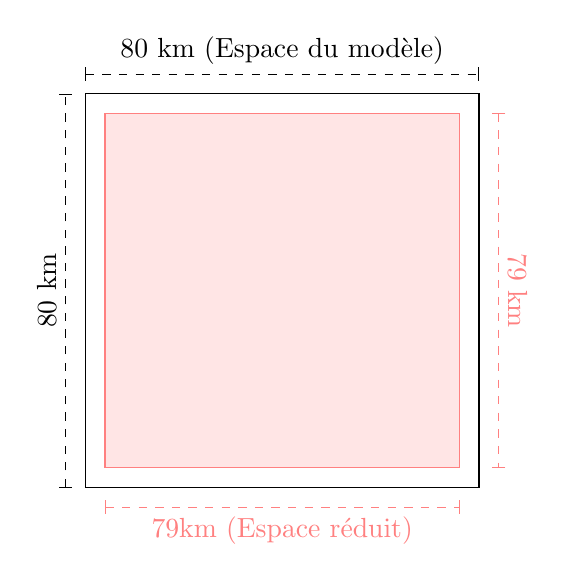
\begin{tikzpicture}[scale=.5]
\draw[] (0,0) -- (0,10) -- (10,10) -- (10,0) -- cycle;
\draw[|-|, very thin, dashed] (0, 10.5) -- node[above] {80 km (Espace du modèle)} (10, 10.5);
\draw[|-|, very thin, dashed] (-0.5, 0) -- node[above, rotate=90] {80 km} (-0.5, 10);

\draw[color=red!50, fill = red!10] (0.5, 0.5) -- (0.5, 9.5) -- (9.5, 9.5) -- (9.5, 0.5) -- cycle;
\draw[|-|, very thin, dashed, red!50] (10.50, 9.50) -- node[above, red!50, rotate=-90] {79 km} (10.5, 0.5);
\draw[|-|, very thin, dashed, red!50] (0.5, -0.5) -- node[below, red!50] {79km (Espace réduit)} (9.5, -0.5);
\end{tikzpicture}
\caption{L'espace support de SimFeodal, un monde théorique.\\
N.B : Dans le schéma, pour une question de lisibilité, les dimensions de l'espace réduit ne sont pas proportionnelles à celles de l'espace d'ensemble.}
\label{fig:espace-simfeodal}
\end{figure}

\paragraph[Endogène]{} Notons enfin que l'espace est strictement \textbf{endogène} au modèle.
On entend par là que le monde n'est pas résultant du chargement d'un fichier géographique ou d'un paramétrage précis : seul un paramètre, qui régit la taille des côtés, joue sur la géométrie de l'espace.
Il nous semble important de le préciser, en particulier parce que c'est, à notre connaissance, assez inhabituel dans la simulation de données géographiques, mêmes théoriques.
Les agents sont en effet placés de manière strictement aléatoire (via un aléa contrôlé tout de même) dans l'espace du modèle, et dès lors, aucune localisation ou surface ne sont identiques ou comparables d'une simulation à l'autre.


\subsubsection{Granularité temporelle}

SimFeodal modélise des processus qui se déroulent sur le temps long, et à ce titre, la gestion de la temporalité y est importante.
Le modèle inscrit son exécution dans une étendue de \textbf{400 ans}, \textbf{discrétisée} sous la forme de 20 pas de temps de \textbf{20 ans} chacun.

\paragraph[Durée]{} La période d'étude, thématique, s'étend entre 800 après J.-C. et 1100, qui correspondent à des repères temporels entre lesquels on estime que le plus gros de la transition étudiée s'est déroulée.
Pour modéliser ces évolutions, nous avons choisi de commencer à la même date, mais de prolonger l'exécution du modèle d'un siècle, portant l'intervalle modélisé à \textbf{400 ans}, \textbf{de 800 à 1200}\footnote{
	Dans les versions précédentes de SimFeodal, \textcite{cura_transition_2017} notamment, cette date était fixée à 1160.
	Nous avons choisi de prolonger de 40 ans parce que cela nous permet de comparer l'état final du modèle au début du XIII$^e$ siècle.
	On obtient de plus un nombre de pas de temps plus \og rond\fg{} (20) qu'auparavant (18), ce qui permet par exemple de représenter l'évolution d'une simulation de manière plus régulière.
}.
Prolonger cette date d'observation permet d'analyser le comportement du modèle après la période d'étude, et par exemple de voir si les processus à l'œuvre subissent bien un ralentissement, marquant par exemple la fin de la féodalité, plutôt qu'un accroissement constant.

\paragraph[Discret]{} Contrairement à la gestion de l'espace, nous avons choisi de modéliser le temps sous forme \textbf{discrète}.
On peut justifier ce choix avec deux raisons principales.
En premier lieu, la transition s'inscrit dans une forte incertitude temporelle. 
Les experts thématiques peuvent certes s'appuyer sur des dates précises, par exemple pour des années de réformes, mais les processus à l'œuvre s'inscrivent dans une durée floue, dont la résolution est difficilement réductible à moins d'un demi-siècle, et à peine meilleure pour des éléments matériels.
Avoir une vision continue du temps s'inscrirait ainsi dans une certaine sur-détermination du modèle en rapport aux connaissances thématiques sur lesquelles il s'appuie.
En second lieu, les processus sont modélisés à la résolution de \og foyers paysans\fg{}, c'est-à-dire à l'échelle de foyers plus que d'individus.
Les migrations des foyers paysans correspondent empiriquement plutôt à des déplacements qui surviennent à l'échelle temporelle de la génération, c'est-à-dire que ces migrations se réalisent en fait quand les descendants d'un foyer s'établissent dans une nouvelle localisation.
La prise en compte d'un temps continu impliquerait donc la mise en place de bien plus de mécanismes probabilistiques, avec des aberrations potentielles plus importantes en terme de trajectoires des agents.

\paragraph[Pas de temps de 20 ans]{} Cette deuxième justification participe au choix de la granularité du modèle. \textbf{Les pas de temps ont une durée de 20 ans}, ce qui correspond à peu près à la durée d'une génération de l'époque.
Cela correspond aussi à la précision globale que l'on peut avoir sur l'apparition d'éléments matériels tels que les églises, paroisses et châteaux\footnote{
Certains de ces éléments sont connus avec une précision bien supérieure, par exemple quand des textes historiques mentionnent leur création.
Ce n'est toutefois pas généralisé, et la granularité moyenne gravite plutôt autour de 20 à 40 ans.
}.
Dans l'ensemble, au vu des connaissances historiques, ces pas de temps doivent être interprétés comme des repères temporels plus que comme des dates précises. 
Que les premiers châteaux apparaissent en 980 ou en 1000 n'a pas d'importance dans le modèle, dans que cela se déroule avant la seconde moitié du XI$^e$ siècle par exemple.


La \cref{fig:frise-chrono} illustre les processus et événements qui surviennent pendant l'ensemble de cette période.

\begin{figure}[H]
	\centering
	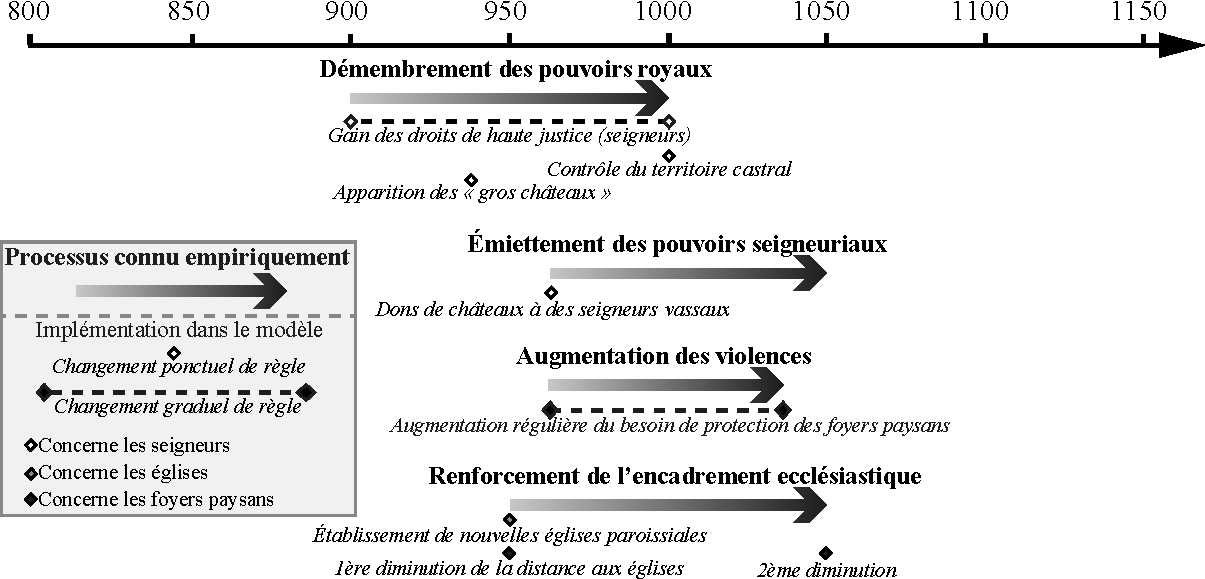
\includegraphics[width=\linewidth]{img/frise_chrono_tmd.pdf}
	\caption{Frise chronologique des processus historiques observés en Touraine implémentés dans SimFeodal. \hl{Figure issue de Peupler la Terre, à corriger/adapter.}}
	\label{fig:frise-chrono}
\end{figure}



\let\orisectionmark\sectionmark
\renewcommand\sectionmark[1]{}%
\section[Fonctionnement général -- \textit{Process overview and schedulling}]{Fonctionnement général\protect\newline \large{\textit{Process overview and schedulling}}\label{sec:fonctionnement-general}}
\orisectionmark{Fonctionnement général}
\let\sectionmark\orisectionmark

SimFeodal est un modèle qui s'inscrit plutôt dans une approche KIDS que KISS (\hl{voir chapitre 1}).
Il est constitué d'une large variété d'agents (\cref{tab:agents-simfeodal}), dotés pour certains de nombreux comportements.
Au total, ce sont près de quarante mécanismes particuliers (ici regroupés en une quinzaine de mécanismes généraux), appelés selon un ordonnancement constant, qui font interagir les agents à chaque pas de temps.
Dans cette partie, nous présentons une synthèse de ces mécanismes, sans entrer dans le détail, algorithmique ou mathématique, de chacun (voir la \cref{sec:meca-specifiques} pour des descriptions plus précises des mécanismes les plus complexes et importants).

\subsection*{Ordonnancement général \label{meca-ordonancement}}

\begin{figure}[H]
	\centering
	% Couleurs
	\definecolor{bleuciel}{HTML}{a6cee3}
	\definecolor{mauve}{HTML}{1f78b4}
	\definecolor{beige}{HTML}{b2df8a}
	\definecolor{vert}{HTML}{33a02c}
	\definecolor{rose}{HTML}{fb9a99}
	\definecolor{rouge}{HTML}{e31a1c}
	% Styles des noeuds et lignes
	\tikzstyle{block} = [rectangle, draw, minimum width=4em, align=center, rounded corners, minimum height=2em, thick]
	\tikzstyle{start} = [draw, circle, minimum height=2em, align=center, thick]
	\tikzstyle{temp} = [very thick, dashed]
	\tikzstyle{line} = [draw, -{Latex[length=2.5mm,width=2.5mm]}]
	\tikzstyle{dline} = [draw, -{Latex[length=2.5mm,width=2.5mm,black!50]}, black!50, densely dotted]
	% 
	\tikzstyle{fps} = [fill=bleuciel]
	\tikzstyle{agregats} = [fill=mauve]    
	\tikzstyle{seigneurs} = [fill=vert]
	\tikzstyle{globals} = [fill=rouge!80]
	\tikzstyle{eglises} = [fill=rose!80]
	\tikzstyle{zps} = [fill=beige]
	\begin{tikzpicture}[node distance = .75cm and .75cm, auto, scale=0.7,every node/.style={transform shape}]
	% Place nodes
	\node [start, fill=rouge!80] (init) at (0,0) {Init.\\du\\monde};
	
	\node [start ,right= of init] (start) {Début\\du tour};
	\node [block, globals,right= of start] (maj-globals) {MaJ des \\variables\\globales};
	\node [block, fps, right= of maj-globals] (renouvellement-fp) {Renouvellement\\des FP};
	\node [block, eglises,right= of renouvellement-fp] (maj-paroisses) {Détection et\\promotions des\\paroisses};
	\node [block, agregats, right = of maj-paroisses] (maj-poles) {Détection\\des\\Pôles};
	
	\node [block, fps, below= of maj-poles] (maj-satisfaction) {MaJ satisfactions des FP};
	\node [block, fps, below=of maj-satisfaction] (migration-fp) {Migration des FP};
	\node [block, seigneurs, temp, below =of migration-fp] (maj-droits) {Gains de \\droits des seigneurs};
	\node [block, seigneurs, below=of maj-droits] (maj-zp) {Collecte des droits};
	
	\node [block, seigneurs, left=of maj-zp] (maj-dons) {Dons droits\\ et châteaux\\des Seigneurs};
	\node [block, globals, temp, left=of maj-dons] (promo-chateaux) {Promotion\\des châteaux};
	\node [block, seigneurs, temp, left=of promo-chateaux] (constructions-chateaux) {Construction\\ de châteaux};
	\node [block, seigneurs, left=of constructions-chateaux] (creation-seigneurs) {Création des\\nouveaux Seigneurs};		
	
	\node [block, agregats, above= of creation-seigneurs] (maj-agregats) {MaJ des Agrégats};
	\node [block, agregats, above=of maj-agregats] (maj-poles2) {MaJ des Pôles};
	\node [block, globals, above= of maj-poles2] (maj-outputs) {MaJ et enregistrement\\des \textit{outputs}};

	
	\path[line]%
	(maj-globals) -- (renouvellement-fp)
	(renouvellement-fp) -- (maj-paroisses)
	(maj-paroisses) -- (maj-poles)
	(maj-poles) -- (maj-satisfaction)
	(maj-satisfaction) -- (migration-fp)
	(migration-fp) -- (maj-droits)
	(maj-droits) -- (maj-zp)
	(maj-zp) -- (maj-dons)
	(maj-dons) -- (promo-chateaux)
	(promo-chateaux) -- (constructions-chateaux)
	(constructions-chateaux) -- (creation-seigneurs)
	(creation-seigneurs) -- (maj-agregats)
	(maj-agregats) -- (maj-poles2)
	(maj-poles2) -- (maj-outputs);

	
	\path[line] (init)-- (start);
	\path[line] (start) -- (maj-globals);
	\path[dline] (maj-outputs)-- (start);	
	\end{tikzpicture}
	\caption[a]{Ordonnancement des mécanismes de SimFeodal.\\
	{\footnotesize
	\colorbox{rouge!80}{\strut Mécanisme global} \colorbox{bleuciel}{\strut Foyers Paysans} \colorbox{rose!80}{\strut Églises} \colorbox{mauve}{\strut Agrégats et Pôles} \colorbox{vert}{\strut Seigneurs} \dbox{\strut Temporaire}
	}
	}
	\label{fig:ordonnancement}
\end{figure}

Dans SimFeodal, les mécanismes sont toujours appelés dans le même ordre (voir \cref{fig:ordonnancement}) : l'ensemble de l'ordonnancement ne change pas tout au long des 20 pas de temps du modèle.
Certains mécanismes sont toutefois temporaires, c'est-à-dire rendus inactifs en fonction des pas de temps : la construction des châteaux, par exemple, n'est pas possible avant 940.
Jusqu'au pas de temps correspondant, le mécanisme est donc désactivé par un paramètre réglable.
Notons que si les mécanismes suivent un ordre déterminé, ce n'est pas le cas des agents qui sont appelés dans chacun de ces mécanismes.
Pour un mécanisme donné, l'ordre d'appel des agents est aléatoire et varie à chaque appel de ce mécanisme.


\subsection{Initialisation \label{meca-init}}

L'initialisation du monde consiste à créer le monde théorique dans lequel les agents vont interagir et à générer ces derniers.
Pendant cette étape, des foyers paysans sont générés dans l'espace du modèle :  une très large proportion est instanciée de manière dispersée et aléatoire.
Quelques dizaines d'agents sont localisés de manière agrégés afin de constituer les premiers agrégats de population, de tailles variables (une vingtaine de villages peu peuplés et quelques petites villes plus importantes, correspondant aux agglomérations secondaires antiques).
Lors de l'initialisation sont aussi créés les premiers seigneurs -- grands seigneurs sans portée spatiale et petits seigneurs localisés aléatoirement dans l'espace -- et les zones de prélèvement dans lesquelles ils prélèveront des droits divers.
L'initialisation est enfin l'occasion de créer et de disperser dans l'espace des églises (150), parmi lesquelles quelques-unes (50) se verront doter de droits paroissiaux et constitueront un premier maillage paroissial.

L'initialisation du monde est appelée une seule fois, avant que les pas de temps ne débutent.
Elle repose fortement sur l'aléatoire, et génère donc une configuration spatiale différente à chaque nouvelle exécution du modèle (voir le paragraphe sur l'endogénéité de la \cref{subsec:reso-spatiale}).
Le détail de l'initialisation est décrit dans une partie ultérieure (\cref{sec:initialisation}), entièrement consacrée à cette étape préliminaire.

\subsection{Variables globales \label{meca-variables}}

Plusieurs mécanismes de SimFeodal dépendent du temps :
la possibilité, évoquée plus haut, pour les seigneurs de construire un château, mais aussi, entre autre, l'évolution des distances que les foyers paysans sont prêts à parcourir pour se rendre à l'église, ce qui permet de formaliser l'impact des réformes grégoriennes.
La mise en place de mécanismes tributaires de dates nous permet ainsi de représenter des événements exogènes au modèle qui peuvent ainsi servir de déclencheurs ou de catalyseurs à des processus de longue durée.
L'incrémentation de la date et la mise à jour des différentes variables temporelles, par exemple en sélectionnant les valeurs de ces différentes variables dans des tableaux de correspondance temporels, constituent donc la première étape de chaque nouveau pas de temps.

\subsection{Renouvellement des foyers paysans \label{meca-renouvellement}}

SimFeodal est un modèle qui simule l'évolution d'un système spatial clôt.
On entend par là qu'il n'y a pas d'échange ou d'interaction avec les régions voisines, ce qui constitue une limite forte, par ailleurs fréquente dans la modélisation géographique.
Pourtant, en particulier dans un modèle mettant en place des migrations, il est difficile de s'abstraire du contexte spatial.
Le monde modélisé constitue certes un système en lui-même, mais aussi un système inscrit comme composante d'un système de peuplement plus large (le royaume des Francs, voire l'Europe du Nord-Ouest).
Nous avons choisi de modéliser les échanges avec l'extérieur par le biais d'un renouvellement partiel des foyers paysans.
A chaque pas de temps, une proportion (5\%) des foyers paysans existant est à cet effet supprimée de la simulation, et une quantité équivalente est réinjectée dans l'espace du modèle.
Afin de ne pas bouleverser l'équilibre de l'agrégation, la localisation dans l'espace suit la proportion de foyers paysans dispersés et agrégés :
s'il y avait 90\% de foyers paysans dispersés avant le renouvellent, 90\% des foyers paysans ré-injectés seront localisés aléatoirement dans l'espace du modèle, et les 10\% restant seront placés dans les agrégats existant\footnote{
Selon un tirage aléatoire pondéré : les agrégats les plus peuplés attireront potentiellement plus de ces nouveaux foyers paysans que les moins peuplés.
Cette logique d'attachement préférentiel (\hl{retrouver où j'en parle si c'est avant}) permet de modéliser l'attractivité qu'exercerait un agrégat peuplé, potentiellement plus connu, sur des foyers paysans venant de régions voisines.
}.

\subsection{Mise à jour du maillage paroissial}

Le moyen-âge voit apparaître un maillage dense, continu dans l'espace, constitué autour d'églises dotées de droits paroissiaux : les paroisses, qui organisent l'ensemble de la vie spirituelle de la population.
Les archéologues ne s'accordent pas sur la date de leur apparition (avant la période étudiée), ni surtout sur le moment où elles constituent un maillage complet (vraisemblablement pendant la période modélisée).
Ils s'accordent cependant sur le rôle de fixation et de stabilisation du territoire qu'elles ont eu \autocite{zadora-rio_paroisses_2008}.
Dans SimFeodal, cette étape de mise à jour du maillage paroissial regroupe en fait trois mécanismes distincts.

\paragraph{Dessin du maillage} Le maillage paroissial est représenté et calculé sous la forme d'une partition de Voronoï autour des églises paroissiales.
On garantie ainsi un pavage complet du territoire, plus lâche dans les zones les moins peuplées et dotées de moins d'églises paroissiales, et plus dense dans les zones les plus peuplées, par exemple dans les agrégats les plus importants qui peuvent être déservis par de nombreuses paroisses ainsi qu'observé empiriquement.

\paragraph{Création de paroisses \og urbaines\fg{}} Dans les agrégats les plus peuplés, certaines paroisses peuvent être amenées à regrouper des centaines de paroissiens, ce qui ne correspondrait pas aux connaissances empiriques.
SimFeodal comprend donc un mécanisme de création de paroisses, via la construction d'églises dotées de droits paroissiaux, au sein des agrégats les plus peuplés, selon une logique probabiliste. 
Plus un agrégat est peuplé, plus il a de probabilités de voir apparaître une nouvelle église paroissiale, dans son étendue, dédiée à sa desserte.

Afin d'éviter l'apparition exponentielle d'églises paroissiales au sein d'un agrégat, cette probabilité est pondérée par le nombre d'églises paroissiales déjà présentes dans l'agrégat.
Ainsi, là où un agrégat constitué de 1~000 foyers paysans et contenant une unique paroisse aura une probabilité de 50\% de voir apparaitre une nouvelle églises paroissiale, un agrégat constitué de 1~000 foyers paysans mais déjà doté de 2 paroisses n'aura qu'une probabilité de 25\%.

\paragraph{Promotion de paroisses \og rurales\fg{}} Tout au long de son développement et à mesure de l'importance sociale qu'il acquière, on sait que le maillage paroissial se densifie, pour parvenir en fin de période au maillage quasi-communal qu'on lui connaît désormais.
Cette densification est observée partiellement dans les zones denses, mais aussi très largement de manière homogène sur le territoire, notamment dans les zones les moins peuplées, afin de garantir un accès facilité aux sacrements à l'ensemble des foyers paysans.
Dans ces zones, on fait apparaître de nouvelles églises paroissiales, soit par promotion d'églises existantes (non dotées de droits paroissiaux), soit par construction de nouvelles églises qui deviendront centres paroissiaux.
Le mécanisme de ces créations est complexe, et on le détaille et l'illustre donc, à l'instar du détail des règles de création de paroisses \og urbaines\fg{}, dans la partie du chapitre relative aux spécificités des mécanismes (\cref{sssec:paroisses}).
Notons simplement que là encore, la promotion ou création d'églises paroissiales en zones peu denses suit une logique de seuil : si une paroisse contient trop de foyers paysans qui en sont suffisamment éloignés (paroisse d'une superficie importante), on tendra à créer une nouvelle église paroissiale plus proche de ces foyers paysans.

\subsection{Détection des Pôles}

Dans SimFeodal, lorsque les foyers paysans migrent, ils sont attirés par des pôles, ensemble composites d'attracteurs (agrégats, églises paroissiales et châteaux), relativement à l'attractivité de ces pôles.
Cette attractivité est relative au nombre et au type d'attracteurs qu'ils contiennent.
Les pôles sont donc indispensables au bon fonctionnement du mécanisme de migration, et leur définition revêt alors une importance nette.
Le mécanisme est encore une fois complexe (voir \cref{sssec:poles} pour le détail), mais on peut le résumer ainsi : un pôle est constitué par la proximité de plusieurs attracteurs, selon une logique de continuité spatiale.
Ainsi, quand une église paroissiale est située à proximité\footnote{
Cette proximité est configurable par le biais d'un paramètre.
Dans SimFeodal, on situe ce seuil à 200 mètres.
} d'un château, lui-même par exemple à proximité d'un agrégat de population, on définit un pôle comme composé par ces trois éléments, et représenté par l'enveloppe convexe formée par leurs géométries.
Afin de ne pas artificiellement diviser des pôles pré-existants, ou au contraire de voir apparaître de nombreux pôles dans un espace restreint (attracteurs séparés de 210 mètres par exemple), on procède ensuite à une fusion des pôles les plus proches.
On considère par exemple qu'un agrégat, quelle que soit son importance, contient et fait partie d'un unique pôle.

Les valeurs d'attractivité des pôles, relatives à leur composition en attracteurs, ont donné lieu à un important travail de paramétrage (\hl{voir chapitre 4, et particulièrement les étapes $n$--$j$}), et est désormais fixée selon ces principes (\cref{tab:attraction-poles}) :

\begin{table}[H]
	\centering
		\caption{Attractivité ($\in [0,1]$) conférée aux pôles par leurs attracteurs.}
	\label{tab:attraction-poles}
	{\renewcommand{\arraystretch}{1.1}%
	\begin{tabular}{|l|l|l|}\hline
		\textbf{Attracteur} & \textbf{Détail} & \textbf{Attractivité} \\ \hline
		\multirow{2}{*}{Châteaux} & Petit & 0.15 \\
		& Gros & 0.25 \\ \hline
		\multirow{4}{*}{Église paroissiale} & 1 & 0.15 \\
		& 2 & 0.25 \\
		& 3 & 0.5 \\
		& 4+ & 0.6 \\ \hline
		\multicolumn{2}{|l|}{Agrégat (doté d'une communauté)} & 0.15 \\ \hline
	\end{tabular}}

\end{table}

\subsection{Satisfaction des Foyers Paysans}

La satisfaction\footnote{
Notons que ce terme n'est pas entièrement \og satisfaisant\fg{} : la migration des foyers paysans est favorisée par une faible satisfaction, c'est-à-dire une absence de satisfaction (qui n'est donc pas un mécontentement ou \og insatisfaction\fg{}), dont l'on retrouve le sens dans le terme anglais \textit{dissatisfaction}.
} des foyers paysans est la condition préalable au mécanisme le plus important de SimFeodal, la migration.
Elle qualifie la capacité des foyers paysans à remplir leurs besoins fondamentaux : \og se nourrir\fg{} (satisfaction matérielle) ; \og assurer son salut\fg{} (satisfaction religieuse) ; et \og éviter d'être l'objet de violences\fg{} (satisfaction \og protection\fg{}) \autocite[Tableau 1, \ppno~309]{cura_transition_2017}.
La satisfaction d'ensemble, qui intervient dans la probabilité de migration, est une synthèse numérique de ces trois satisfactions spécifiques.
Ces composantes ne sont pas hiérarchisées, sinon en considérant qu'elles sont normalisées \og par le bas\fg{} : le satisfaction d'ensemble est égale à la plus faible de ses trois composantes, pondérée par l'appartenance à une communauté, laquelle procure un contre-pouvoir face aux différentes pressions subies par les foyers paysans.

Le détail des calculs est donnée dans la partie dédiée (\cref{sssec:satisfaction}), mais on peut toutefois déjà expliciter les choix de modélisation de chacune des composantes de la satisfaction d'ensemble.

\paragraph{Satisfaction matérielle}

Dans SimFeodal, on considère la satisfaction matérielle comme une fonction des différentes redevances dont un foyer paysan doit s'acquitter : plus il doit régler de droits, moins il est satisfait.
Comme pour la satisfaction générale, notons que l'appartenance ou non à une communauté intervient dans ce calcul.
On estime en effet que les communautés (paysannes, rurales, villageoises\ldots) permettent de constituer une force suffisante pour exercer un véritable contre-pouvoir face à des seigneurs qui seraient trop exigeants.

\paragraph{Satisfaction religieuse}

La satisfaction religieuse représente la capacité d'un foyer paysan à se rendre facilement à l'église pour y assister aux différents sacrements (baptêmes, mariages, eucharistie\ldots) qui rythment la vie spirituelle de l'époque.
Dans SimFeodal, cette capacité est modélisée comme une fonction de la distance à l'église paroissiale la plus proche : plus on est éloigné d'une église paroissiale, plus la satisfaction est faible.
Les seuils de distance définissant le \og loin\fg{} et le \og proche\fg{} évoluent au cours du temps, afin de représenter l'alourdissement des obligations religieuses tout au long de la période, par exemple à l'occasion des réformes grégoriennes.

\paragraph{Satisfaction de \og protection\fg{}}

Avec la diminution du pouvoir de l'autorité centrale carolingienne assortie d'un émiettement des pouvoirs locaux, la région d'étude subit un regain de violences militaires.
L'apparition des châteaux forts en est l'un des symptômes représentatifs.
De la même manière que la satisfaction religieuse dépend de la distance aux églises, on considère dans SimFeodal que la satisfaction \og protection\fg{} des foyers paysans dépend de la distance au château le plus proche.
Un château assure ainsi une certaine protection à la population.
Cette protection se montre de plus en plus critique au fur et à mesure de l'avancement de la période et donc du modèle.
Comme pour la satisfaction religieuse, les seuils de distance évoluent au cours du temps, de même ici que le \og besoin de protection\fg{}, qui permet de renforcer l'augmentation nette du climat de violence au cours de la période.

\subsection{Migration des Foyers Paysans \label{meca-migration}}

La satisfaction, décrit ci dessus, sert de condition probabiliste à la possibilité pour les foyers paysans de migrer.
Rappelons que les pas de temps durent 20 ans : les migrations ne sont pas des déplacements quotidiens ou saisonniers, mais illustrent plutôt le déménagement et le choix de localisation que chaque nouvelle génération de paysans est amené à réaliser.
Dans SimFeodal, nous considérons que les foyers paysans suffisamment satisfaits ne sont pas amenés à migrer.
On migre quand on est insatisfait, et l'on cherche alors à augmenter sa satisfaction.
L'implémentation de cette logique suit un mécanisme probabiliste, où l'insatisfaction augmente la probabilité de migrer.
Le détail du mécanisme de migration est complexe et sera détaillé dans la \cref{sssec:migration}.
Notons aussi que ce mécanisme est sans doute le plus important et impactant du modèle SimFeodal : à ce titre, il a subit de très nombreux changements depuis le début de la conception du modèle, tel qu'illustré dans \hl{le chapitre 4}.

Dans cette version de SimFeodal, la migration répond à une succession de conditions.
Dans l'ensemble, quand les foyers paysans migrent, c'est nécessairement vers un pôle, et si possible un pôle plus attractif que celui dans lequel ils seraient.
Cette migration peut prendre deux formes :
\begin{itemize}
	\item une migration \og locale\fg{}, où les foyers paysans cherchent des pôles plus attractifs dans un rayon défini (2~500 mètres) ;
	\item et la migration \og lointaine\fg{}, où au contraire les foyers paysans cherchent un agrégat\footnote{
		\textit{N.B.} : La migration locale se fait en direction d'un pôle (qui peut ou non contenir un agrégat), alors que la migration lointaine vise un agrégat, potentiellement plus important.
	} situé au delà du rayon local.
\end{itemize} 
La migration locale est privilégiée sur la migration lointaine, qui, en simplifiant, ne s'exerce que quand la première n'est pas possible (absence de pôles locaux, tirages de probabilité échoués etc.).

Notons que ces règles ne s'appliquent pas à l'identique à tous les foyers paysans : une part de ceux-ci (20\%), intitulés \og non mobiles\fg{}, n'ont pas la possibilité d'effectuer des migrations lointaines.
Ils sont restreints à des migrations locales, ce qui permet de modéliser le comportement de dépendances de certaines catégories de population historiques (les serfs et esclaves, qui n'avaient pas le droit de quitter le domaine de leur seigneur, par exemple).


\subsection{Gains de droits}

Au fur et mesure de l'avancement de la période, le pouvoir central s'efface et les ressorts locaux subissent un émiettement important, voyant apparaître de nombreux seigneurs de moindre importance (les chevaliers notamment).
Ces seigneurs gagnent et s'arrogent le prélèvement de nouveaux droits (droits banaux, droits de basse justice etc.), augmentant d'autant la charge fiscale dont doivent s'acquitter les foyers paysans.

Dans SimFeodal, cela est modélisé sous la forme de l'apparition constante de nouvelles zones de prélèvement par l'intermédiaire desquelles les seigneurs pourront prélever de nouveaux droits.
Cela peut concerner de nouveaux seigneurs, lors de leur apparition dans l'espace du modèle, ou au contraire se faire au bénéfice de seigneurs plus anciens.
Du point de vue de l'implémentation, ce comportement est formalisé sous la forme d'une probabilité ($0.15$), pour les petits seigneurs, de créer une nouvelle zone de prélèvement autour de leur localisation, à chaque pas de temps.

Ce mécanisme s'associe à une autre, majoritairement exercé par les grands seigneurs, qui leur permet de prélever, à partir d'une date donnée (voir \cref{meca-variables}), des droits de haute justice.
Cela est là encore effectué à partir d'un tirage de probabilité ($P = 0.2$ pour les grands seigneurs de 900 à 1000 et $1$ après; $P = 0.2$ pour les petits seigneurs châtelains à partir de 1000).

\subsection{Collecte des droits}

Dans SimFeodal, les droits sont prélevés au travers de représentations géographiques de leur emprise spatiale\footnote{
Notons bien qu'il s'agit d'un choix de modélisation, c'est-à-dire ici d'une simplification forte.
Les droits au moyen âge n'avaient pas nécessairement de logique spatiale : ce pouvait être en fonction de l'usage d'un matériel (four banal, moulin\ldots), ou en fonction d'une appartenance familiale (la \og taille\fg{} personnelle) par exemple, sans que la localisation précise n'entre en jeu.
} : les zones de prélèvement.
Celles-ci sont de trois types (cf. \cref{tab:agents-simfeodal}), qui correspondent à trois grandes catégories de droits connus : les droits fonciers ; les droits de haute justice ; et les autres droits, qui regroupent une forte diversité de redevances locales (droits banaux, droits de basse et moyenne justice, droits locaux\ldots).

Dans SimFeodal, chaque droit a ses propres modalités de collecte (voir le détail en \cref{sssec:collecte-droits}).
On peut résumer cela de manière géométrique : les zones de prélèvement sont des cercles de rayon variables, qui se superposent et s'intersectent très largement.
Chacune de ces zones de prélèvement appartient à un seigneur, qui l'a créée, et peut en plus être confiée en garde à un autre seigneur (voir le paragraphe suivant).
Les seigneurs (propriétaires et gardiens) prélèvent des droits aux foyers paysans situés dans les zones de prélèvement.
Plus ces derniers sont situés dans une région dense en zones de prélèvements, plus ils seront amenés à s'acquitter de nombreux droits, et plus leur satisfaction matérielle sera faible.
Pour les seigneurs, à l'inverse, plus les redevances collectées seront importantes (plus ils posséderont de zone de prélèvement recouvrant de nombreux foyers paysans), plus leur puissance sera importante, ce qui leur permettra notamment de construire des châteaux, gages de renommée et de revenus accrus.

\subsection{Dons entre seigneurs \label{meca-dons}}

On a mentionné que les seigneurs pouvaient se voir confier des zones de prélèvement en garde.
Historiquement, cela correspond à la pratique de certains seigneurs de nommer des gestionnaires ou de distribuer des terres à des seigneurs de moindre importance pour s'assurer de leur vassalité.

Dans SimFeodal, les seigneurs peuvent donner en gardiennage, selon une probabilité, chacune de leurs possessions : zones de prélèvement et châteaux.
Dans le premier cas, les seigneurs récipiendaires sont choisis de manière privilégiée dans le voisinage des seigneurs donateurs : on favorise ainsi une transmission locale.
Pour les châteaux, il n'y a pas de préférence locale, mais seuls des seigneurs de faible importance peuvent être récipiendaires, c'est-à-dire ceux qui ne sont pas déjà châtelains (ie. qui n'ont pas déjà de château en propre ou en garde).

En donnant en garde leurs propriétés, les seigneurs se garantissent la constitution d'un réseau de vassalité (non modélisé) et accroissent leur puissance symbolique.
Dans SimFeodal, on le modélise en augmentant les redevances que les seigneurs collectent dans les zones de prélèvement données en gardiennage : le seigneur gardien collecte les redevances classiques, alors que le seigneur suzerain collecte ces mêmes redevances accrues d'un léger facteur\footnote{
Par exemple, un seigneur collecte une puissance (symbolique) de $1$ sur les foyers paysans dont il collecte les droits fonciers.
En nommant un \og gardien\fg{}, il y collectera $1.25$ de puissance, et le vassal récupèrera lui $1$. Voir le détail dans le \cref{tab:puissance-droits}.
}.
Notons que ces dons n'ont pas d'influence sur la satisfaction des foyers paysans : pour eux, seul un seigneur (le gardien, ou le propriétaire quand la zone n'a pas été confiée en gade) prélève les droits.
Le mécanisme de collecte n'est donc pas symétrique : les seigneurs y gagnent plus que ce que les foyers paysans n'y \og perdent\fg{}.

\subsection{Promotion des châteaux}

De nombreux châteaux ont été construits pendant la période étudiée.
Il y avait naturellement une forte hétérogénéité dans leur ampleur, leur importance stratégique et le degré de protection qu'ils apportaient.

Dans SimFeodal, on a choisi de simplifier cette hiérarchie en distinguant deux types de châteaux : les \og petits châteaux\fg{} et les \og gros châteaux\fg{}.
Les gros châteaux ont un pouvoir d'attraction plus développé (cf. \cref{tab:attraction-poles}), renforçant l'attraction des pôles qu'ils constituent et par là même accroissant la probabilité de voir se développer à proximité des agrégats majeurs.
Lors de leur création (voir \textit{infra}), les châteaux sont toujours des \og petits châteaux\fg{}.
Le mécanisme de promotion, probabiliste, permet à un château situé dans un pôle important (c'est-à-dire constitué de plusieurs attracteurs : agrégat, églises paroissiales) de devenir \og gros château\fg{}, et renforce encore l'attrait de ce pôle déjà avantageux.

\subsection{Construction de châteaux}

Tout au long de la période, de nouveaux châteaux sont construits et renforcés. C'est l'apparition des \og châteaux forts\fg{}.
Si l'on connaît des châteaux préalables à la période étudiée, leur démultiplication survient surtout à partir de la seconde moitié du X$^e$ siècle.
Ils sont surtout construits par les grands seigneurs existants afin de mailler le territoire d'un réseau de protection, même si certains sont aussi l'œuvre de seigneurs de moindre envergure qui se sont enrichis pendant la période en profitant du système féodal.
En Touraine, on considère que la majeure partie des châteaux forts ont été construits entre le X$^e$ et le XIII$^e$ siècle, et que leur production a ensuite fortement ralenti.
Les châteaux sont bâtis en bonne partie dans des villes déjà attractives, même si l'on observe aussi quelques créations dans des espaces peu peuplés, qui tendront alors à le devenir par la suite (les bourgs castraux).


Dans SimFeodal, on fait apparaître les châteaux de manière endogène, en considérant qu'il n'y en a aucun au début de la période.
À partir de 940, les seigneurs ont la possibilité de créer des châteaux.
Cette possibilité est basée sur une probabilité, fonction de la puissance des seigneurs, c'est-à-dire de l'accumulation des redevances perçues à chaque pas de temps.
Plus la puissance d'un seigneur est importante, plus il a de chances de pouvoir créer un château.
Cette probabilité est aussi fonction de la puissance relative des seigneurs : au fur et à mesure que le temps passe et que de nouveaux seigneurs émergent, les grands seigneurs historiques voient leur importance relative décliner, et leur probabilité de créer de nouveaux châteaux diminuer en conséquence.
A contrario, certains petits seigneurs favorisés par leurs prélèvements et par les gardiennages reçus peuvent, de manière exceptionnelle, être amenés à bâtir eux-aussi des châteaux.
Afin de ne pas voir l'apparition de zones concentrant de nombreux châteaux, nous avons mis en place une restriction spatiale à leur implantation.
Un nouveau château ne peut ainsi être construit à moins de 5 km d'un château existant.
On garanti ce faisant une répartition spatiale non aberrante au regard des connaissances empiriques.

Notons qu'en matière d'ordonnancement, la construction des châteaux a lieu après le calcul de la satisfaction protection des foyers paysans, de la promotion en gros châteaux, et aussi après le don de ces mêmes châteaux, ce qui pourrait sembler contre-intuitif.
Ce choix a été fait pour symboliser la durée de construction des châteaux, bien plus longue que les autres phénomènes d'apparition décrits dans le modèle : un château apparaît en fin de tour, il n'est donc pas véritablement utilisable avant le tour suivant, soit 20 ans plus tard.
Les détails du mécanisme, notamment en ce qui concerne les probabilités différentes pour les petits et les grands seigneurs, ou encore les choix de localisation des nouveaux châteaux (au sein d'un agrégat ou non par exemple), sont explicités dans la partie dédiée (\cref{sssec:constru-chateaux}).

\subsection{Création de nouveaux seigneurs}

L'émiettement des pouvoirs pousse à l'apparition de nombreux seigneurs, d'envergure très locale majoritairement, tout au long de la période.
On estime qu'il y avait une vingtaine de seigneurs en Touraine en début de période et plus de 200 en 1200.
Ces seigneurs sont détenteurs d'un faible pouvoir, peu disposant de terres conséquentes : une large proportion tire ses revenus de terres et d'installations octroyées par leur suzerain, par exemple sous la forme de banalités.

Dans SimFeodal, l'accroissement des seigneurs est modélisé sous la forme de l'apparition, à chaque pas de temps, d'un nombre légèrement aléatoire de nouveaux seigneurs, dont la variation est mesurée de manière à obtenir environ 200 seigneurs en fin de simulation.
Parmi ces seigneurs, seule une faible proportion (10\%) est dotée de terres et collecte donc des droits fonciers.
Les autres seigneurs constituent un vivier potentiel de récipiendaires de dons divers (voir \cref{meca-dons}).
L'ensemble de ces seigneurs sont répartis, spatialement, au sein d'agrégats existants.

\subsection{Détection des agrégats \label{meca-agregats}}

L'un des constats forts ayant mené à l'identification d'une \og transition\fg{} \autocite{pumain_convergences_2017, nuninger_cadre_2017} dans le système de peuplement de l'Europe du Nord-Ouest est la hiérarchisation du système de peuplement.
Dans ce cadre, on la constate par une concentration de la population dispersée, et par l'apparition de hameaux, villages et petites villes suivant une hiérarchie de population.
L'utilisation de ces termes plus spécifiques est particulièrement sensible en histoire et en archéologie, en particulier en raison de potentiels anachronismes.
Nous avons donc choisi de ne pas discrétiser le continuum représentatif de l'agglomération de foyers et de le dénommer, dans son sens le plus littéral, \og agrégat\fg{} de population.

Dans SimFeodal, ces agrégats sont interprétés de manière morphologique, à l'instar des agglomérations de l'INSEE : est agrégat un regroupement d'au moins 5 foyers paysans, espacés l'un à un autre d'au plus 100 mètres.
Cette définition permet de représenter des entités géographiques très diverses, depuis le petit agrégat composé de quelques foyers paysans à l'agrégat majeur, semblable à une petite ville, constitué de plusieurs centaines de foyers.
L'agrégat est une entité spatiale au sens propre, dotée par exemple de ses propres attributs et sa propre emprise spatiale, constituée par l'enveloppe convexe des foyers paysans qui le composent : c'est une entité individuelle mais composite.

Certains agrégats peuvent contenir une \og communauté\fg{}, c'est-à-dire une structure institutionnalisée gérée par les foyers la composant et qui procure un avantage en matière de rapport de force et de subsistance matérielle (par exemple avec les logiques de gestion collective des terres et outils que permettent les communautés agraires).
Dans SimFeodal, les agrégats ont une probabilité (20\%), à chaque pas de temps, de voir apparaître une communauté en leur sein.
D'un point de vue informatique, cela complexifie énormément la détection des agrégats : dès lors que des agents ont des propriétés propres, celles-ci doivent être transmissibles dans le temps, c'est-à-dire d'un pas de temps à l'autre.
Pourtant, la détection des agrégats est renouvelée à chaque pas de temps, ce qui signifie qu'un agrégat détecté en 900, situé au même endroit qu'un agrégat de 880, ne peut que difficilement lui être associé\footnote{C'est un problème récurrent des méthodes de \textit{clustering} dynamique que de réussir à mener des associations entre les \textit{cluster} de différentes dates.}.
Le mécanisme spécifique de détection, de constitution et de transmission des attributs des agrégats est donc particulièrement complexe, et fait l'objet d'une présentation détaillée plus loin dans le chapitre (\cref{sssec:agregats}).

\subsection{Actualisation des pôles}

La détection des pôles intervient relativement tôt dans l'ordonnancement des mécanismes.
Il est par exemple nécessaire que les pôles soient définis avant le mécanisme de migration des foyers paysans, qui dépend en partie de ces pôles.
Pourtant, en vue de préparer et de sauvegarder les \textit{outputs}, il est nécessaire de redéfinir les pôles, qui ont notamment été affectés par les modifications dans les agrégats et châteaux.
Cela permet par exemple, lors de l'enregistrement des sorties, de conserver un lien entre un agrégat et le pôle dans lequel il se situe, notamment pour étudier les relations entre composition des pôles et populations des agrégats qui y sont attachés.
Dans SimFeodal, nous sommes alors obligés, afin d'avoir des sorties exploitables, de reconstruire les pôles en fin de tour.
Cette duplication d'un mécanisme est malheureuse et peu optimale, mais rendue nécessaire par la structure des différents mécanismes précédents et en particulier par l'interdépendance qui caractérise de nombreux types d'agents dans le modèle.

\subsection{Enregistrement des \textit{outputs} \label{meca-outputs}}

Lors de la conception et du développement de SimFeodal, on a rapidement choisi de mener l'exploration du modèle très largement \textit{a posteriori} (\hl{voir chapitre 5, section 5.2.1}) de l'exécution du modèle.
L'enregistrement des données d'un modèle est un problème complexe, dont les enjeux et difficultés sont largement résumées dans le chapitre 5 (\hl{section 5.1}).
Notons ici, tout de même, que nous avons besoin d'enregistrer des données relatives à l'ensemble des agents, pris individuellement, et à leurs attributs.
Les données produites par la simulation sont par conséquent assez massives et revêtent une importance particulière.
Lors de cette phase, des variables globales et spécifiques sont actualisées, des indicateurs synthétiques sont calculés, et l'ensemble des données subit des traitements voués à en simplifier la conservation, par exemple en réduisant la précision des nombres décimaux\footnote{
Pour illustrer l'importance de ce traitement d'apparence anecdotique, on peut prendre l'exemple de l'enregistrement des géométries.
Celles-ci, dans la plate-forme Gama \autocite{taillandier_building_2018} utilisée pour SimFeodal, sont exportées dans un format textuel normalisé, le \og Well-Known Text\fg{} (\textit{WKT}).
Par défaut, chaque géométrie est décrite avec une précision de 12 chiffres décimaux, soit une résolution spatiale proche du picomètre, l'ordre de grandeur des atomes.
Cette précision n'a strictement aucune utilité dans un modèle où les ordres de grandeur minimums tournent autour des dizaines et centaines de mètres.
D'un point de vue informatique, stocker 12 décimales au lieu d'entiers démultiplie considérablement la place nécessaire pour l'enregistrement des données.
Ces étapes de simplification sont donc indispensables pour disposer d'un modèle fonctionnel et exploitable.
}.



\let\orisectionmark\sectionmark
\renewcommand\sectionmark[1]{}%
\section[Concepts de modélisation-- \textit{Design concepts}]{Concepts de modélisation \protect\newline \large{\textit{Design concepts}}}
\orisectionmark{Concepts de modélisation}
\let\sectionmark\orisectionmark

Cette section du protocole ODD vise à mettre en avant les concepts courants de la modélisation de systèmes complexes qui sont employés dans le modèle.
C'est une liste exhaustive, et l'ensemble des concepts décrits n'ont pas nécessairement de correspondance dans SimFeodal.
Par soucis de clarté, on décrira donc d'abord les grands principes de modélisation qui nous semblent fondamentaux dans SimFeodal, et ensuite, le cas échéant, les ensembles de concepts mobilisés.

\subsection{Principes de base - \textit{Basic principles}}

\paragraph{\textit{Space Matters}}

SimFeodal est un modèle intrinsèquement spatial.
De nombreux modèles agents mobilisent l'espace, ou au moins une représentation ou un support présent dans le concept du \og monde\fg{} virtuel répandu en modélisation agent, quand bien même l'approche n'est pas foncièrement spatiale.
Par exemple, on trouve de nombreux modèles de réseaux dans les bibliothèques classiques de modèles agents, où l'espace support est une vue planaire plus qu'un support euclidien ou topographique réel.

Dans SimFeodal, au contraire et comme la brève description des mécanismes le montre, une très large partie des (inter)actions dépendent des distances (modèles de types gravitaires pour le calcul de la satisfaction religieuse et de protection), des contextes spatiaux (évaluation de l'environnement local pour les migrations locales) ou encore des voisinages (constitution d'agrégats, détection des pôles etc.).
SimFeodal n'est donc pas qu'un modèle qui prend appui sur l'espace, mais un modèle dont le fonctionnement inhérent est spatial, voir géographique ou géométrique.
\textit{Space matters}\ldots

\paragraph{\textit{Push-Pull}}

L'évolution de la structure spatiale que l'on observe dans SimFeodal résulte de la migration des foyers paysans, qui tendent ainsi à se concentrer.
Ce mécanisme est fortement inspiré et ancré dans une certaine pratique de modélisation, courante dans le champ des études de mobilité résidentielle, que l'on peut qualifier de \og \textit{push-pull}\fg{} \autocite{tannier_analyse_2017}.
On entend par là que les agents subissent un double mécanisme, répulsif, qui les pousse à déménager (ou migrer dans SimFeodal), le \textit{push}, et attractif, qui conditionne leur choix de destination à l'attractivité d'un lieu, le \textit{pull}.
Ce modèle est d'ordinaire mobilisé dans l'étude de mobilités résidentielle, ou encore vis-à-vis de pratiques quotidiennes de l'espace.
Son application nous semble inédit sur des processus d'une temporalité plus importante, telle que le temps long sur lequel SimFeodal s'appuie.

Si ce choix peut paraître surprenant, il résulte avant tout d'une certaine \og culture de modélisation\fg{}, l'une des co-conceptrices du modèle ayant une forte habitude de modélisation de dynamiques résidentielles (\textit{ibid.}).
En dehors de l'importance de cette \og path-dependency\fg{} d'un modèle aux conceptions préalables de ses modélisateurs, notons tout de même que ce type de modélisation nous semble assez facilitateur de dialogue avec des experts thématiques.
Cela permet peut-être plus simplement que d'autres paradigmes de passer d'une connaissance experte spécifique à une modélisation plus générique.

\paragraph{Attachement préférentiel} Ce \og grand concept\fg{} est le dernier sur lequel SimFeodal s'appuie, quoi que de manière bien moindre que les deux précédents.
Il est néanmoins mobilisé, sous une forme faible, en matière de concentration : les pôles les plus importants attirent plus, et peuvent voir se développer des agrégats et des églises paroissiales qui à leur tour augmenteront leur attractivité.
Cela concoure à des logiques de renforcement des plus forts et d'amoindrissement (relatif) des plus faibles.
Notons qu'un mécanisme d'attachement préférentiel aboutit a une distribution log-normale de ses composantes \autocite{barabasi_emergence_1999}, ce qui pourrait être le cas ici concernant les tailles des agrégats.
Pourtant, dans SimFeodal, l'attachement préférentiel n'est pas directement fonction de la taille des agrégats, et est limité par certains seuils (le nombre de paroisses est par exemple limité dans la prise en compte de l'attractivité d'un pôle).
Nous ne pouvons alors en aucun cas prédire -- ni même estimer selon un raisonnement intuitif -- que la forme d'attachement préférentiel implémentée dans SimFeodal doit entraîner une hiérarchisation forte (log-normale) des agrégats. 

\subsection{Théories et concepts de la modélisation agents mobilisés}

Le protocole ODD définit un ensemble de \textit{design concepts} qui peuvent être mobilisés dans la conception d'un modèle à base d'agents.
Pour chacun de ces 10 concepts (voir \cref{tab:proto-ODD}\footnote{
Il nous semble que les dénominations de ces concepts ne sont pas extrêmement claires et intuitives.
Nous recommandons au lecteur de plutôt chercher à les comprendre en lisant les exemples de questions donnés dans la colonne de droite du tableau.
}), nous décrivons donc brièvement, le cas échéant, si et comment ils sont appliqués dans SimFeodal.

\paragraph{Émergence} Ce mécanisme constitue l'un des fondements de nombreux modèles complexes, et SimFeodal n'y échappe pas.
La diversité des éléments analysés dans le modèle est trop importante pour faire une liste des éléments qui y émergent (\hl{voir le chapitre 3, section 3.? par exemple}), et l'on peut prendre pour exemple les modifications de structure spatiale des foyers paysans.
Les foyers paysans ne communiquent ni n'interagissent directement les uns avec les autres, et pourtant ils tendent à se regrouper en formant des agrégats dont la hiérarchie augmente avec le temps du modèle.
Dans ce cas spécifique, il y a donc une émergence \og forte\fg{}, puisque les structures résultantes de l'agrégation des foyers paysans sont attractives alors que les foyers paysans en eux-mêmes ne le sont pas.

\paragraph{Adaptation} Dans SimFeodal, ce concept n'est pas présent au sens littéral : les agents ne s'adaptent pas à un environnement en modifiant leur comportement.
L'adaptation est toutefois présente dans un sens plus évolutionniste, darwinien.
On peut en effet considérer que les agents les mieux positionnés au départ seront ensuite avantagés tout au long de la simulation.
On peut prendre l'exemple d'un seigneur situé à proximité d'un agrégat qui aurait tendance à devenir important, qui verrait ainsi sa puissance augmenter de manière exponentielle.
L'action peut aussi être indirecte : ce seigneur, par sa puissance acquise, avantagerait aussi les seigneurs de son voisinage (dons de droits par exemple).

Notons aussi que la description de ce concept interroge la capacité des agents à chercher à maximiser une mesure de réussite.
Dans ce sens là, on peut parler d'adaptation pour les foyers paysans : plutôt que de chercher à maximiser leur satisfaction, on peut tout de même dire qu'ils essaient, à force de tirages aléatoires, de ne pas la minimiser.


\paragraph{Objectifs} Nous répondons ici à la seconde partie de la description :\\
\og When individuals make decisions by ranking alternatives, what criteria do they use?\fg{} (\textcite{grimm_documenting_2017}, voir \cref{tab:proto-ODD}).\\
Dans SimFeodal, un mécanisme stochastique pondéré est mobilisé de nombreuses fois pour établir la destination d'un foyer paysan, lors d'un renouvellement (voir \cref{meca-renouvellement}) ou d'une migration locale ou lointaine (\cref{meca-migration}): la \og loterie pondérée\fg{}.
Dans ce mécanisme, les foyers paysans \og choisissent\fg{} leur agrégat (ou leur pôle) de destination en fonction de l'attractivité de celui-ci :
plus un agrégat/pôle est attractif, c'est-à-dire composé de nombreux foyers paysans (ou attracteurs), plus il est susceptible d'attirer.
Chaque agrégat/pôle, y compris le moins attractif, a toutefois une probabilité, faible, d'attirer de nouveaux foyers paysans.
Le classement d'attracteurs en fonction de leurs caractéristiques propres est donc très présent dans SimFeodal.
Notons qu'il l'a de plus été plus encore dans des versions préalables du modèle, où la distance était prise en compte de concert à l'attractivité, formant un véritable modèle gravitaire microscopique pour chaque choix de (re-)localisation des foyers paysans.

\paragraph[Learning \& Prediction]{} Les deux concepts suivants, l'apprentissage (\textit{\textbf{learning}}) et la prédiction (\textit{\textbf{prediction}}), ne nous semblent pas adaptés à la description de SimFeodal.

\paragraph{Perception - \textit{Sensing}} En tant que tel, les agents de SimFeodal n'ont aucune perception de leur environnement, c'est-à-dire qu'ils n'ont aucun comportement \og actif\fg{} de mise à jour de leurs connaissances, ni d'utilisation quelconque de connaissances d'ailleurs.
Par extension, toutefois, on peut trouver des notions de connaissances globales ou locales chez les agents par la manière dont certains mécanismes sont construits.
Par exemple, chez les foyers paysans, la migration peut être locale ou globale. 
En cas de migration locale, la recherche de destinations potentielles se fait dans le voisinage des foyers paysans.
On pourrait alors y voir une notion de perception, et y considérer que ces foyers paysans (ou les foyers paysans non mobiles, les serfs) ont une perception uniquement locale de leur environnement, contrairement aux autres foyers paysans qui auraient une connaissance globale du monde modélisé.

\paragraph{Interaction} C'est un concept qui est souvent au cœur de nombreux modèles à base d'agents.
Dans SimFeodal, il n'y a pourtant que peu d'interaction au sens propre, c'est-à-dire impliquant un échange, une communication ou une transaction quelconque entre des agents.
Cela est légèrement faux dans le cas des seigneurs, qui peuvent donner en garde leurs droits et châteaux à d'autres seigneurs.
La non-réciprocité de l'échange ou encore l'absence d'\fg{}association\fg{}\footnote{
	C'est-à-dire que pour un seigneur donateur, le choix de son vassal n'a aucune importance et aucun impact dans le modèle, et réciproquement.
} nous poussent toutefois à ne pas considérer ces mécanismes comme des mécanismes d'interaction proprement dite.
On pourrait, de manière figurée, voir de l'interaction entre les foyers paysans en considérant la constitution des agrégats : les agents n'interagissent pas directement ensemble, mais c'est leur co-présence qui est facteur de définition d'une entité de niveau supérieur\footnote{
A mettre au regard de la célèbre définition de la ville de \textcite{levy_ville_2003} : \og Géotype de substance sociétale fondé sur la coprésence\fg{}.
}.
\setcounter{savefootnote}{\value{footnote}}

\paragraph{Stochasticité} Dans les parties précédentes de ce chapitre, on a plusieurs fois mentionné l'importance de la stochasticité dans SimFeodal.
Celle-ci est omniprésente : dès l'initialisation du monde (\cref{meca-init}), la distribution des foyers paysans, agrégats, églises et seigneurs est entièrement aléatoire.
En parcourant l'ensemble du déroulement de SimFeodal (\cref{fig:ordonnancement}), on réalise qu'à l'exception des détections spatiales (agrégats, pôles et paroisses) et de l'enregistrement des sorties, tous les mécanismes comportent une part important de stochasticité.
On le constate \textit{a minima} sur l'ordre d'appel des agents (\cref{meca-ordonancement}), et de manière bien plus importante dans d'autres mécanismes (loteries pondérées, probabilités de migration, probabilité de construction et de localisation de châteaux\ldots).
Conjuguée avec la complexité du modèle, c'est-a-dire l'imbrication des mécanismes qui rend leur comportement non linéaire, la stochasticité concoure à faire de SimFeodal un modèle profondément complexe et aléatoire.
On ne peut prédire le comportement du modèle, ni même l'effet de certains paramètres (\hl{voir le chapitre 6, section analyse de sensibilité, ou chapitre 3 sur l'évaluation des params}), sans le simuler.


\paragraph{Collectifs} Cette partie de la grille de lecture ODD interroge l'existence et la constitution de \og collectifs\fg{}, c'est-à-dire d'agrégats d'entités individuelles, ainsi que la manière dont ils sont implémentés : dotés
d'attributs propres ou enrichissant les attributs des entités constituantes.
\\
Dans SimFeodal, on pense directement aux agrégats, entités de niveau mésoscopique constituées de foyers paysans.
Les agrégats ont leurs attributs propres, qui dépendent toutefois largement des foyers paysans (attractivité, emprise spatiale).
Les agrégats ont toutefois une caractéristique propre, la présence d'une communauté ou non.
Cette caractéristique joue, de manière rétroactive, sur les foyers paysans qui composent l'agrégat puisque la présence d'une communauté dans leur agrégat augmente mécaniquement la satisfaction matérielle et générale des foyers paysans.

Une autre entité mésoscopique est constituée par la proximité d'attracteurs (églises paroissiales, châteaux et agrégats de population), qui dessinent alors des pôles composites.
Comme pour les agrégats, certains attributs des pôles dérivent directement des attracteurs les composants, par exemple leur géométrie.
L'autre propriété des pôles, leur attractivité, dépend aussi directement des attracteurs qui les composent, sans toutefois que la relation soit strictement cumulative : une cinquième église paroissiale n'apportera pas d'attractivité au pôle dont elle fait partie (voir \cref{tab:attraction-poles}).

\paragraph{Observation} Ce dernier \og design concept\fg{} nous semble quelque peu incongru et dissonant au regard des autres concepts déployés.
Il s'agit ici de définir les données produites et collectées par le modèle à base d'agents.
Nous avons en partie mentionné le type d'enregistrement des données (\cref{meca-outputs}), et déjà annoncé que cet aspect fondamental de SimFeodal serait couvert très largement dans des parties dédiées, cette problématique occupant une large partie du \hl{chapitre 5}.

Pour aider au positionnement de SimFeodal vis-à-vis de modèles à base d'agents classiques, on peut toutefois expliciter ici que la collecte des données est indispensable dans SimFeodal, puisque le modèle est pensé pour être analysé \textit{a posteriori}, requérant l'analyse simultanée de nombreux indicateurs hétérogènes.
SimFeodal est ainsi un modèle dont l'un des objectifs est de produire des données, lesquelles permettront de comprendre le modèle ultérieurement, au contraire d'un modèle essentiellement dynamique et \og animé\fg{} tel que celui de Schelling, où le modèle peut être appréhendé en direct de son exécution. 


\let\orisectionmark\sectionmark
\renewcommand\sectionmark[1]{}%
\section[Situation initiale -- \textit{Details - Initialisation}]{Situation initiale\protect\newline \large{\textit{Details - Initialisation}}\label{sec:initialisation}}
\orisectionmark{Situation initiale}
\let\sectionmark\orisectionmark

\subsection{Une situation initiale théorique et endogène}

L'une des spécificités de SimFeodal, comme indiqué dans la \cref{subsec:reso-spatiale}, est que l'initialisation est strictement endogène au modèle.
Elle constitue donc un premier \og sous-modèle\fg{} de SimFeodal, chargé de générer le monde dans lequel les agents évolueront.
Dans l'ordre, l'initialisation consiste en l'exécution de 4 mécanismes : (1) création des foyers paysans ; (2) création des églises ; (3) mise à jour des agrégats ; (4) création des seigneurs.

La création des églises (2) est assez simple : on répartie, de manière aléatoire dans l'espace du modèle, 150\unskip\astfootnote{Ce nombre est paramétrable.\label{ftn:nombre-parametrable}} églises.
Puis, parmi ces églises, on en tire aléatoirement 50\footref{ftn:nombre-parametrable} a qui l'on attribue des droits paroissiaux.

Le mécanisme de création des premiers seigneurs (4) est lui aussi assez évident : là encore, on répartit, de manière toujours aléatoire, un nombre donné de grands seigneurs\footref{ftn:nombre-parametrable}.\\
On localise aussi, selon un aléa contraint, un ensemble\footref{ftn:nombre-parametrable} de petits seigneurs au sein des agrégats existants, lesquels ont été délimités selon le mécanisme standard (voir \cref{meca-agregats}).
Les petits seigneurs générés se voient directement associés à une zone de prélèvement de type \og foncier\fg{}, de rayon et de taux de prélèvement aléatoires bornés : dès l'initialisation, les premières zones de prélèvement sont donc créées.

La création des foyers paysans (1) est plus complexe, notamment car elle doit être aléatoire tout en respectant une structure choisie par les modélisateurs via les paramètres.
Dans l'ensemble, elle se déroule en trois phases :
\begin{enumerate}
	\item On crée des \og petites villes\fg{}, peuplées d'une trentaine\footref{ftn:nombre-parametrable} de foyers paysans situés dans une voisinage suffisant pour être identifiable en tant qu'agrégat.
	\item On répète le processus pour des \og villages\fg{}, peuplés de 10\footref{ftn:nombre-parametrable} agents.
	\item On répartie alors de manière aléatoire l'ensemble des autres foyers paysans, c'est-à-dire le nombre total souhaité\footref{ftn:nombre-parametrable} auquel on retranche les foyers paysans créés dans une petite ville ou dans un village, dans l'espace du modèle.
\end{enumerate}
Afin que les foyers paysans constitutifs des villes et villages soient assurés de former des agrégats (3), la répartition des foyers paysans qui les composent suit une logique itérative illustrée dans la \cref{fig:init-fp}.

\begin{figure}[H]
	\centering
	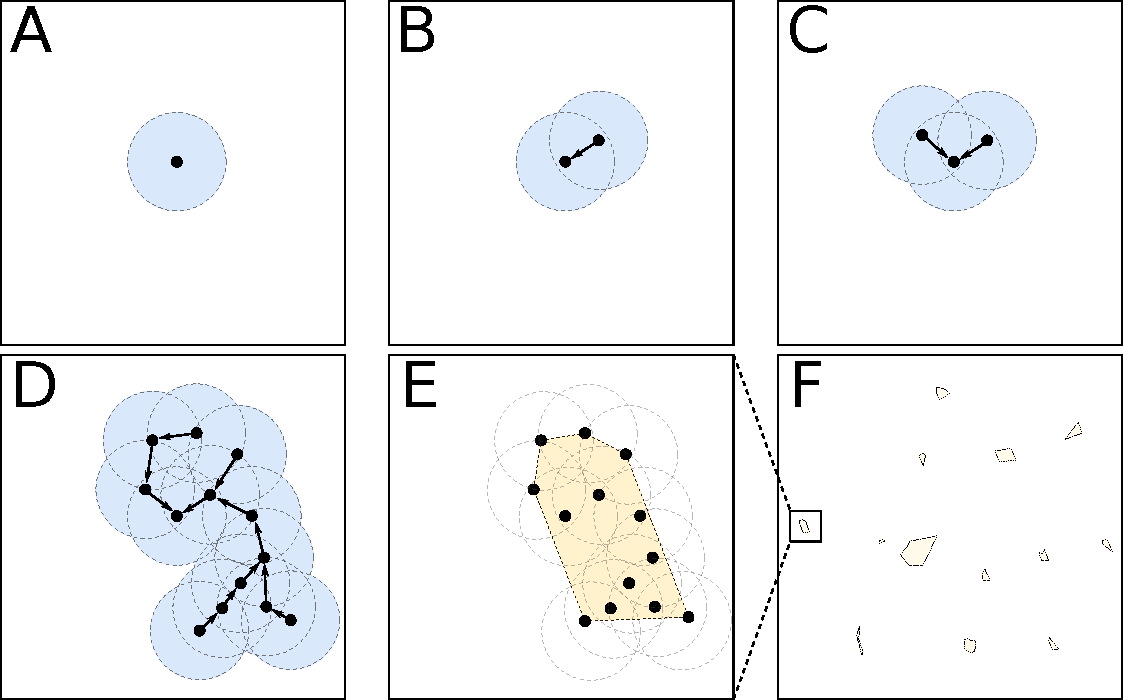
\includegraphics[width=.98\linewidth]{img/init_fp.pdf}
	\caption{Étapes successives de l'initialisation des foyers paysans agrégés (petites villes et villages).\\
	(A) On génère un foyer paysans ;
	(B) on génère un nouveau foyer paysan dans un rayon donnée du premier ;
	(C) et (D) on continue à générer de nouveaux foyers paysans dans le rayon de n'importe lequel des foyers existants ;
	(E) la géométrie d'un agrégat correspond à l'enveloppe convexe des foyers paysans ;
	(F) en fin d'initialisation, tous les agrégats initiaux sont répartis dans le monde.}
	\label{fig:init-fp}
\end{figure}



\subsection{Paramètres d'initialisation}

Dans la partie précédente, on a plusieurs fois indiqués que certaines des valeurs numériques de l'initialisation étaient paramétrables, c'est-à-dire qu'on peut les faire varier afin de générer des structures spatiales initiales différentes.
Cela participe à l'endogénéisation de l'espace support de SimFeodal, où il n'y a aucun \og \textit{input}\fg{}, mais un ensemble de paramètres régissant les différents sous-modèles.
Pour l'initialisation, les paramètres sur lesquels on peut jouer pour tester différents scénarios sont précisés dans le \cref{tab:params-initiaux}.


\begin{table}[H]
	\centering
		\caption{Paramètres permettant de contrôler l'initialisation du monde de SimFeodal.}
	\label{tab:params-initiaux}
	{\renewcommand{\arraystretch}{1.25}%
	\begin{tabular}{|M{2cm}|M{4cm}|m{5.25cm}|m{1.25cm}|}
		\hline
		\textbf{Sous-mécanisme} & \textbf{Paramètre} & \textbf{Intitulé} & \textbf{Valeur} \\ \hline
		\makecell{Création\\du monde} & Taille du monde & taille\_cote\_monde & 80 km \\ \hline
		\multirow{7}{*}{\makecell{Génération\\des\\Foyers\\Paysans}} & Nombre total de FP & init\_nb\_total\_fp & 4000 \\ \cline{2-4} 
		& Nombre de petites villes & init\_nb\_agglos & 8 \\ \cline{2-4} 
		& Nombre de FP par petite ville & init\_nb\_fp\_agglo & 30 \\ \cline{2-4} 
		& Nombre de villages & init\_nb\_villages & 20 \\ \cline{2-4} 
		& Nombre de FP par village & init\_nb\_fp\_village & 10 \\ \cline{2-4} 
		& Distance d'agrégation des FP & distance\_detection\_agregat & 100 m \\ \cline{2-4} 
		& Taux de FP \og dépendants\fg{} (ie. non mobiles) & proba\_fp\_dependant & 20\% \\ \hline
		\multirow{2}{*}{\makecell{Génération\\des\\Églises}} & Nombre total d'églises & init\_nb\_eglises & 150 \\ \cline{2-4} 
		& (dont) Nombre d'églises paroissiales & init\_nb\_eglises\_paroissiales & 50 \\ \hline
		\multirow{3}{*}{\makecell{Génération\\des\\Seigneurs}} & Nombre de Grands Seigneurs & init\_nb\_gs & 2 \\ \cline{2-4} 
		& \makecell{Puissance relatives\\des Grands Seigneurs} & \makecell{puissance\_grand\_seigneur$1$ \\ \textelp{} \\ puissance\_grand\_seigneur$N$} & 50\% \\ \cline{2-4} 
		& Nombre de Petits Seigneurs & init\_nb\_ps & 18 \\ \hline
	\end{tabular}}

\end{table}



\let\orisectionmark\sectionmark
\renewcommand\sectionmark[1]{}%
\section[Données en entrée -- \textit{Input data}]{Données en entrée\protect\newline \large{\textit{Input data}}}
\orisectionmark{Données en entrée}
\let\sectionmark\orisectionmark

Comme indiqué, il n'y a pas véritablement d'\textit{inputs} dans SimFeodal : tout est paramètre, et dès lors dynamique.
En même temps, le modèle comporte de très nombreux paramètres : entre une quarantaine et une soixantaine selon les définitions possibles de ce qu'est un paramètre, voir \hl{chapitre 4}.\\
On peut donc voir dans la multiplicité des paramètres une proximité avec la notion de données en entrée, qui ne s'expriment toutefois pas sous la forme traditionnelle.

Par exemple, pour mettre en place des comportements exogènes permettant de faire varier le modèle à différentes dates précises, on peut classiquement faire appel à des données de sortie d'un autre modèle, ou à un fichier de configuration.
Dans SimFeodal, cette logique est bien présente, mais est gérée directement au sein du modèle, sans faire appel à des données externes.
Certains paramètres prennent ainsi la forme de tableaux d'associations (aussi appelés dictionnaires, ou \og \texttt{map}\fg{} en informatique), qui mettent en correspondance des valeurs de paramètres à des dates précises (voir \cref{lst:maps-gama}).
\medskip

{\footnotesize
\begin{lstlisting}[caption={
Deux exemples de \texttt{map} dans Gama.
\textit{À partir de 800, les églises doivent se situer entre 5 et 25~km, puis entre 3 et 10~km de 960 à 1060, et entre 1.5 et 5~km après cette date.}}, captionpos=b, label={lst:maps-gama}]
map<int,int> dist_min_eglise <- [800::5000,  960::3000,  1060::1500];
map<int,int> dist_max_eglise <- [800::25000, 960::10000, 1060::5000]; 
\end{lstlisting}
}

Pour respecter le formalisme ODD que suit ce chapitre, on peut au final considérer que SimFeodal est un modèle qui ne repose sur aucune donnée en entrée.
Conceptuellement, le rôle joué par les paramètres du modèle s'en approche toutefois assez fortement.
Le \hl{chapitre 4} permet d'éclairer cette description en entrant plus en détail dans la définition et la nomenclature des paramètres.

\let\orisectionmark\sectionmark
\renewcommand\sectionmark[1]{}%
\section[Mécanismes spécifiques -- \textit{Submodels}]{Mécanismes spécifiques\protect\newline \large{\textit{Submodels}}\label{sec:meca-specifiques}}
\orisectionmark{Mécanismes spécifiques}
\let\sectionmark\orisectionmark


\subsection{Introduction}

Cette partie du chapitre est plus technique, et vise à présenter précisément différents mécanismes de SimFeodal évoqués dans la partie relative au fonctionnement général du modèle (\cref{sec:fonctionnement-general}).
On ne vise ici pas l'exhaustivité, les détails d'implémentation étant bien trop nombreux pour être entièrement explicités.
Cela ferait un double-emploi assez conséquent en sus du code-source du modèle disponible à la consultation (voir l'\hyperlink{avant-propos}{avant-propos}).

Notons aussi que la présentation des mécanismes n'est pas nécessairement exacte, c'est-à-dire une description fidèle de la manière dont les mécanismes sont implémentés informatiquement sous forme de codes-sources.
Nous avons ici fait le choix de présenter les mécanismes sous la forme, discursive et schématique, la plus courte et compréhensible, quand bien même cette forme n'est qu'une \og équivalence\fg{} de la réalité de l'implémentation.
Ces écarts entre présentation discursive des mécanismes et implémentation effective sont discutés dans l'\cref{enc:polarite-implementation}.

On remarquera enfin que avons préféré présenter ces spécifiques dans un ordre différent de celui de l'ordonnancement dans le modèle (cf. \cref{fig:ordonnancement}), en les regroupant plutôt par les types d'agents concernés par chacun.
On présentera d'abord les mécanismes \og globaux\fg{}, c'est-à-dire relevant de la détection des agrégats, pôles et des logiques de promotion et création de paroisses ; puis les mécanismes relatifs au foyers paysans ; et enfin ceux impliquant l'action des seigneurs.

\bigskip 
\begin{encadre}{Écarts entre présentation et implémentation}{polarite-implementation}
	
La présentation des mécanismes d'un modèle ne suit pas toujours la manière dont ces mécanismes sont implémentés dans le code-source d'un modèle.
C'est naturellement vrai entre deux \og domaines\fg{} d'un modèle (si l'on reprend la triade des domaines conceptuels, empirique et implémenté de \textcite{livet2014diversite}), au vu des écarts qu'il peut y avoir par exemple entre le modèle conceptuel et le modèle implémenté.
Toutefois, cela peut aussi se produire au sein d'un même domaine, par exemple ici pour le \og domaine du modèle\fg{}, c'est-à-dire dans l'implémentation du modèle.
La présentation discursive d'un modèle suit ses règles propres, par exemple la nécessité de suivre une progression linéaire, quand bien même faite d'allers-retours.
L'implémentation informatique, au contraire, ne suit pas forcément les mêmes règles, et tend même à requérir des logiques très différentes au nom d'une \og optimisation\fg{} du code-source, propre à chaque langage informatique.
Dans cet encadré, nous souhaitons mettre en avant trois types de processus où la présentation discursive et l'implémentation effective sont différentes tout en produisant des résultats équivalents.
Ces types de processus ne visent pas l'exhaustivité, mais sont des exemples rencontrés dans la présentation du modèle faite dans ce chapitre.

\paragraph{Perspective de l'implémentation} Quand un tirage aléatoire probabiliste est appliqué sur un grand nombre d'entités, son espérance théorique tend vers une fréquence empirique, en vertu de la loi des grands nombres.
En simulation à base d'agents, cela signifie que choisir une proportion de 10\% d'une large population (\og probabilité de groupe\fg{}) est quasi-équivalent à doter chacun des individus d'une probabilité de $0.1$ d'être choisis (\og probabilité individuelle\fg{}).
Cette équivalence est fortement mobilisée dans SimFeodal, la \og perspective\fg{} -- probabilité individuelle ou de groupe -- changeant parfois à plusieurs reprises dans un même mécanisme, selon la praticité ou la performance (informatique) de l'une ou l'autre.
Dans la description du modèle, où on essaie d'avoir la vision la plus \og agent-centrée\fg{} possible, on présentera préférentiellement des mécanismes comme faisant appel à des probabilités individuelles, quand bien même l'implémentation effective se baserait sur une approche proportionnelle, mobilisant des probabilités de groupe.

\paragraph{Factorisation} Une autre différence tient à l'ordre d'exécution des sous-mécanismes par un ensemble d'agents.
En mathématiques, $k\times (x+y)$ est égal, selon les règles de factorisation, à $k{\cdot}x + k{\cdot}y$.
Dans un système multi-agents, la logique est la même, quand bien même l'ordre d'appel des agents peut faire varier le résultat et l'on considère donc à nouveau qu'il s'agit d'une équivalence plus que d'une égalité : les programmes \ref{lst:facto1} et \ref{lst:facto2} sont équivalents.\bigskip

\noindent\begin{minipage}[b]{.45\textwidth}
	\begin{lstlisting}[caption={Factorisé},frame=tlrb, captionpos=b, label = {lst:facto1}]
ask agents [
  do A;
  do B;
]
	\end{lstlisting}
\end{minipage}\hfill
\begin{minipage}[b]{.45\textwidth}
	\begin{lstlisting}[caption={Développé},frame=tlrb, captionpos=b, label = {lst:facto2}]
ask agents [
  do A; ]
ask agents [
  do B; ]
	\end{lstlisting}
\end{minipage}

En terme d'efficacité du code, à nouveau, l'alternance entre ces approches d'implémentation permet de résoudre certaines difficultés d'implémentation plus simplement.
On peut ainsi factoriser les calculs légers et au contraire développer, pour faciliter le stockage intermédiaires entre autre, les calculs plus lourds.
Pour bien différencier les étapes successives, dans le cadre d'une description discursive, il sera souvent plus aisé de présenter les sous-processus de manière développée plutôt que factorisée, ce qui, encore une fois, n'implique rien quant à l'implémentation réelle.

\paragraph{Optimisation} Les deux types de processus précédents peuvent être combinés, pour répondre à des questions d'optimisation informatique, c'est-à-dire par exemple permettre au modèle de fonctionner plus rapidement en fonction des spécificités des langages informatiques choisis.
Dans Gama, par exemple, il est plus lent, informatiquement, de calculer la distance depuis 1000 agents à 10 agents, que l'inverse, quand bien même les résultats sont ici strictement identiques.
Par exemple, le calcul de la satisfaction de protection des foyers paysans demande à chacun de mesurer sa distance au château le plus proche.
Il est bien plus rapide de calculer, depuis la perspective des châteaux, la distance aux différents foyers paysans en en prenant le minimum.
Dans cet exemple, l'implémentation se fait dans un sens opposé à celui du discours, sans que cela n'ait la moindre conséquence -- au niveau du domaine conceptuel, empirique, ou même en termes de mécanisme implémentés --, sinon une plus grande optimisation du fonctionnement informatique du modèle.
\end{encadre}

\subsection{Mécanismes globaux}

\subsubsection{Identification des agrégats \label{sssec:agregats}}
	
\begin{figure}[H]
	\centering
	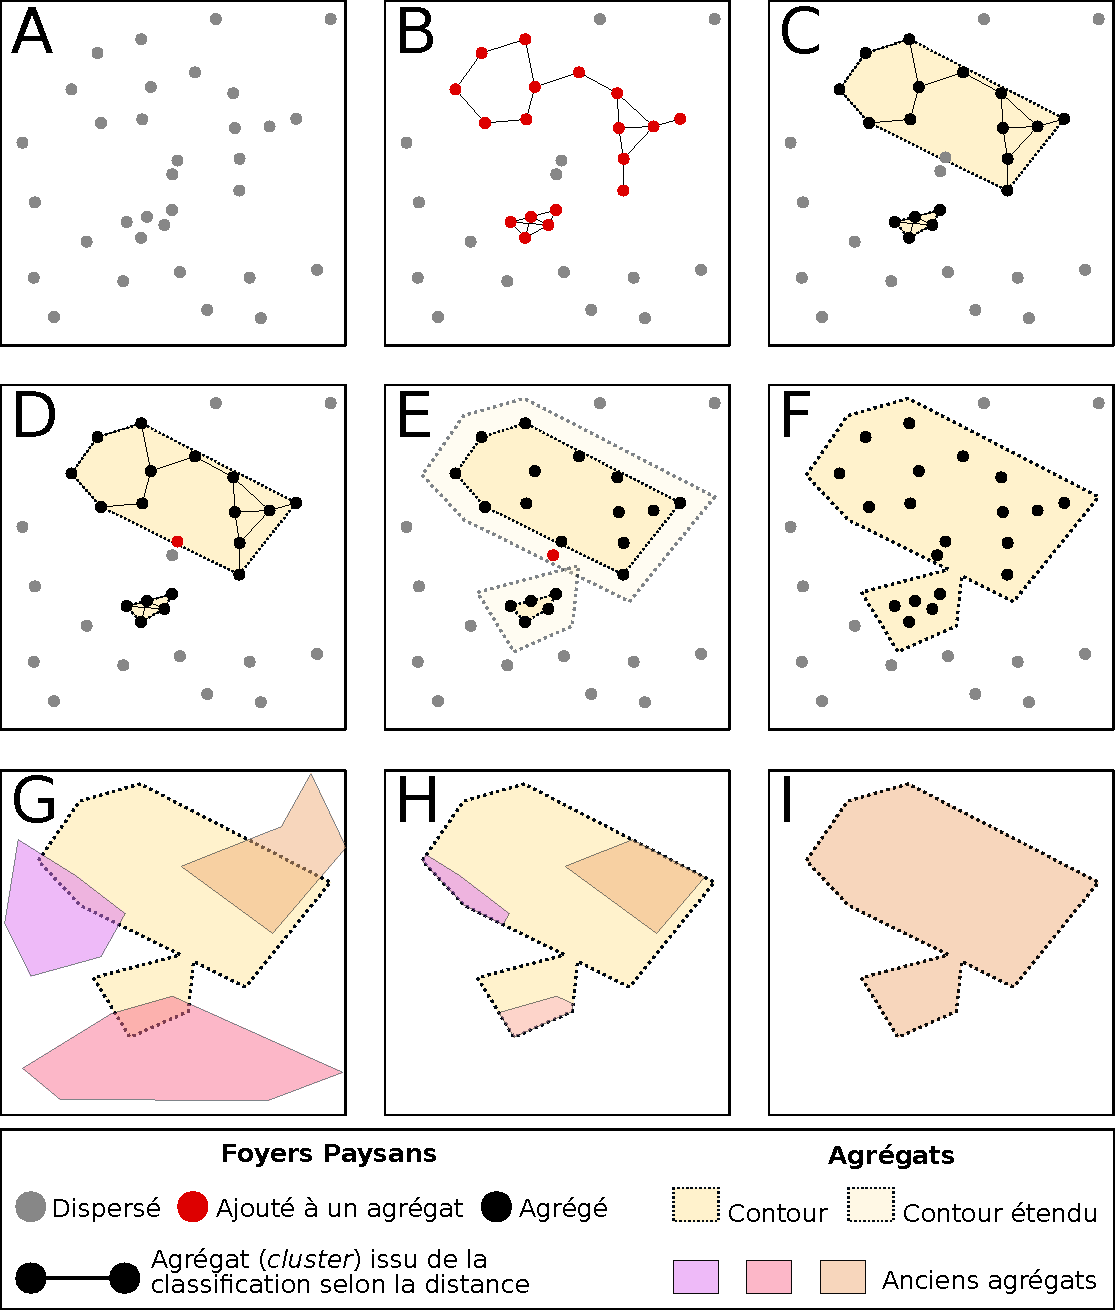
\includegraphics[width=.75\linewidth]{img/detection_agregats.pdf}
	\caption{Détection et de l'héritage des agrégats.}
	\label{fig:detection-agregats}
\end{figure}

La \cref{fig:detection-agregats} présente les étapes successives de détection des agrégats.
À chaque pas de temps, on repart d'une situation \og neutre\fg{}, c'est-à-dire que tous les foyers paysans sont considérés comme dispersés (\textbf{A}).
On exécute un algorithme de classification basé sur la distance\footnote{
L'opérateur Gama \textsf{simple\_clustering\_by\_distance}, proche conceptuellement de l'algorithme DBSCAN.
} : les \textit{clusters} constitués d'au moins 5 foyers paysans espacés de moins de 100~m sont considérés comme des agrégats(\textbf{B}).
On fixe alors la géométrie des agrégats, qui prend la forme de l'enveloppe convexe des foyers paysans qui les composent (\textbf{C}).
Les foyers paysans inclus dans la surface d'un agrégat y sont ajoutés (\textbf{D}).
On crée ensuite des \textit{buffers} de 100~m autour des agrégats et on y rattache à nouveau les foyers paysans inclus dans la surface (\textbf{E}).
Dernière étape dans la détection des agrégats, pour ne pas multiplier les agrégats proches les uns des autres, on procède à une étape de fusion : on réalise l'union géométrique des agrégats qui s'intersectent (\textbf{F}).\\
Les trois dernières étapes concernent la transmission des propriétés des agrégats à travers les pas de temps, et en particulier de la présence ou non d'une communauté en leur sein.
On isole les agrégats du pas de temps précédent qui intersectent les nouveaux agrégats (\textbf{G}).
On procède ensuite à une intersection entre les géométries de ces anciens agrégats et le nouvel agrégat (\textbf{H}).
Le nouvel agrégat hérite alors des propriétés de l'ancien agrégat dont la superficie d'intersection est la plus importante, c'est-à-dire l'agrégat orange ici (\textbf{I}).
	
	\subsubsection{Identification des pôles \label{sssec:poles}}

\begin{figure}[H]
	\centering
	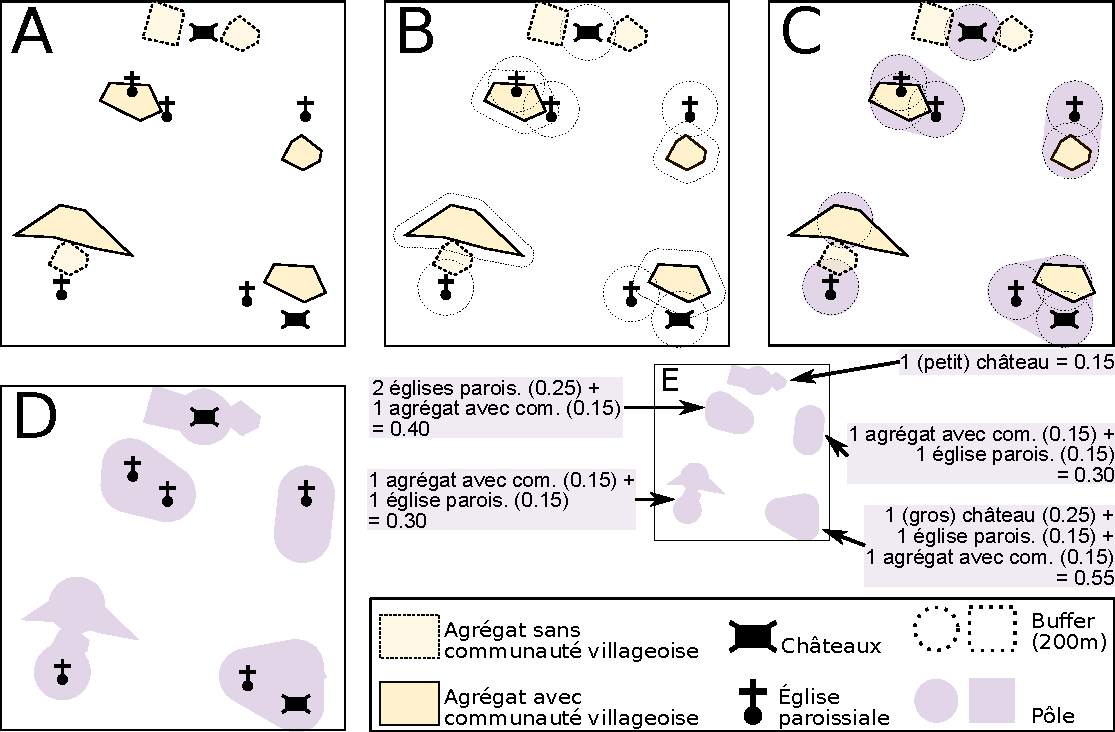
\includegraphics[width=\linewidth]{img/detection_poles.pdf}
	\caption{Les étapes du mécanisme de détection et de calcul d'attractivité des pôles.}
	\label{fig:detection-poles}
\end{figure}

Les pôles sont des agents composés d'attracteurs de trois types : les châteaux (petits et gros), les églises (uniquement celles dotées de droits paroissiaux) et les agrégats (uniquement ceux comportant une communauté paysanne).
Les pôles et leur délimitation spatiale revêtent une importance particulière lors de la migration des foyers paysans : ils attirent d'autant plus que leur attractivité est importante, et le cas échéant, les foyers paysans migrants s'installent à l'intérieur de leur délimitation.
La \cref{fig:detection-poles} illustre la méthode de définition spatiale des pôles, ainsi que des exemples de calcul de leurs attractivités.

À chaque pas de temps, on repart d'une situation \og neutre\fg{}, c'est-à-dire que l'on recalcule systématiquement les pôles sans repartir des pas de temps précédents (\textbf{A}).
On commence par identifier les attracteurs situés à moins de 200~m les uns des autres (\textbf{B}) pour identifier les pôles : ceux-ci peuvent être constitués de plusieurs attracteurs proches, ou d'un unique attracteur.
L'enveloppe spatiale des pôles est définie comme un \textit{buffer} de 200~m autour de l'enveloppe convexe formée par le centroïde des attracteurs qui les composent (\textbf{C}).
Il s'agit par conséquent d'un cercle de rayon de 200~m pour les pôles mono-attracteurs, et d'un polygone pour les pôles composites.
Afin de renforcer la probabilité de voir croître les agrégats à proximité des pôles, on fusionne (union géométrique) l'enveloppe spatiale des pôles avec les contours de l'ensemble des agrégats (comportant ou non une communauté paysanne) intersectés.
Cela permet à des pôles peu éloignés de fusionner à leur tour (\textbf{D}).
On peut alors calculer leur attractivité en se reportant au \cref{tab:attraction-poles} (p.~\pageref{tab:attraction-poles}) (\textbf{E}).


	
	\subsubsection{Création et promotion d'églises paroissiales \label{sssec:paroisses}}
	
	\begin{figure}[H]
		\centering
		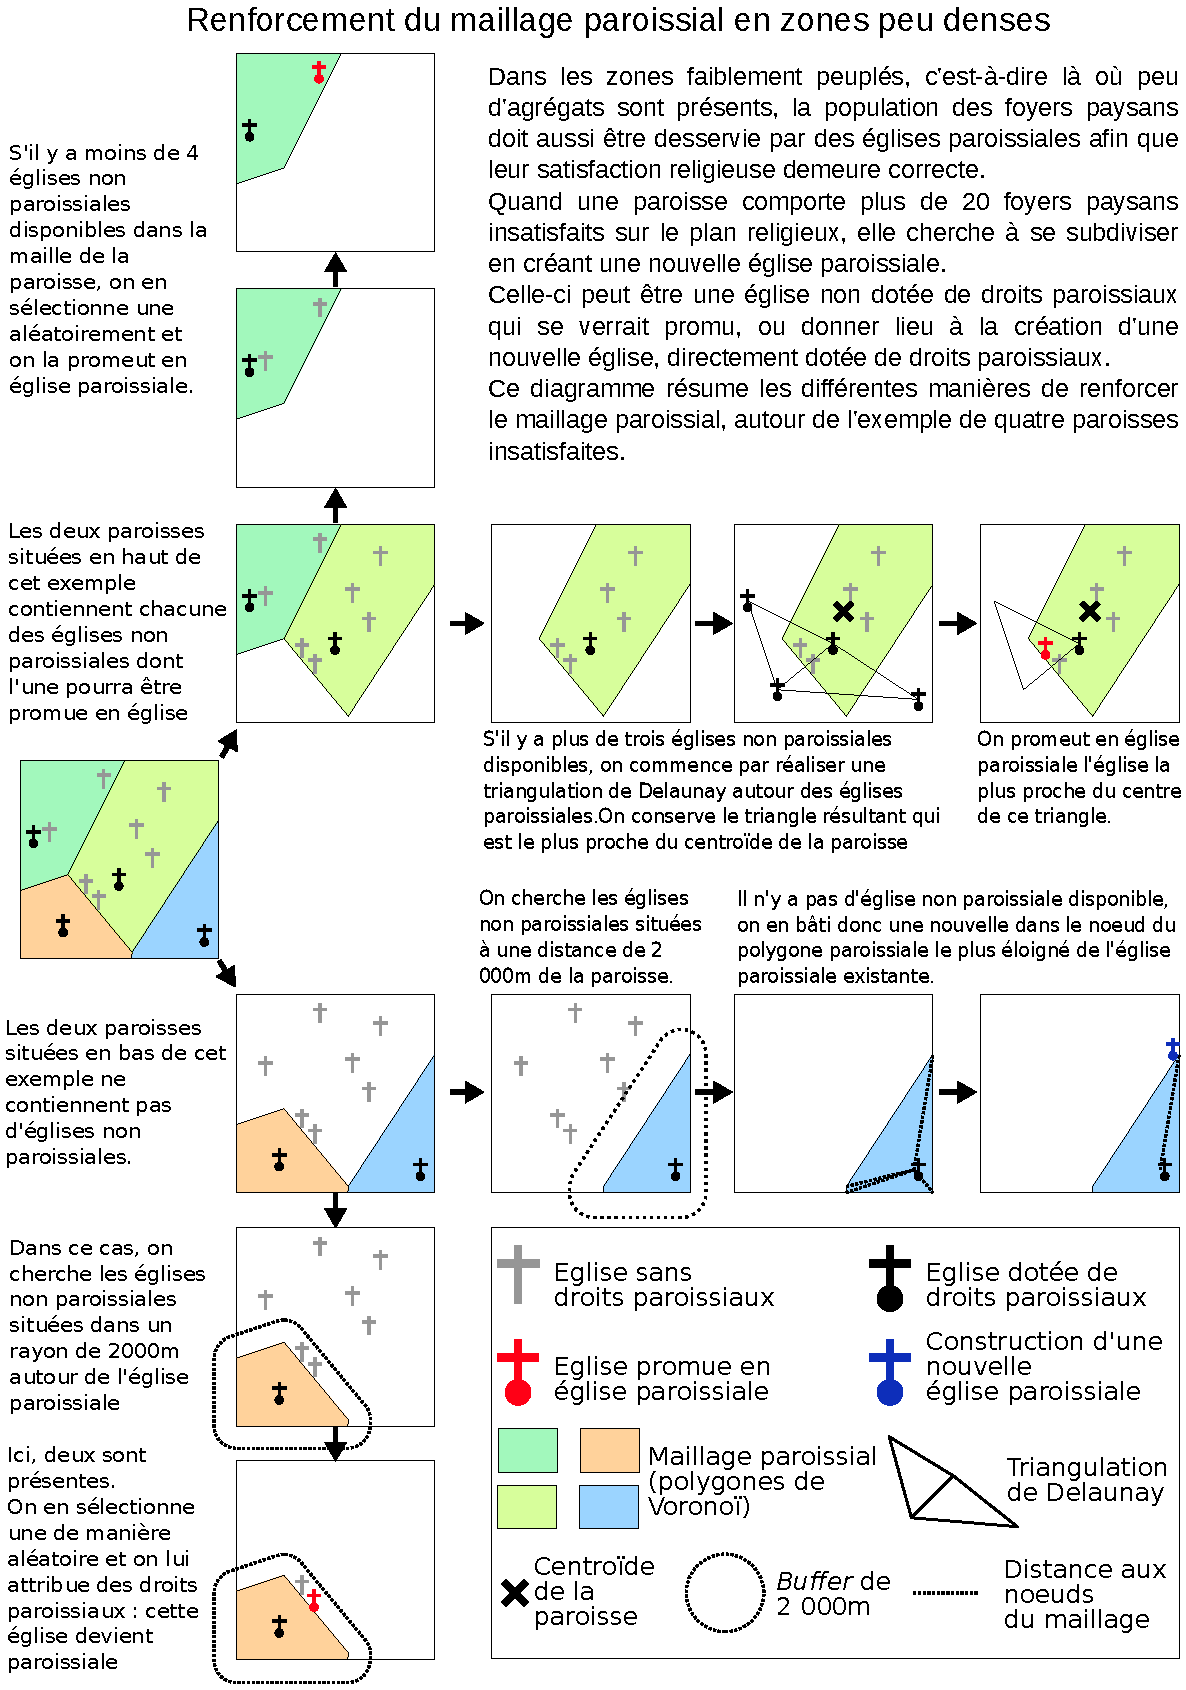
\includegraphics[width=1\linewidth]{img/constru-promo_paroisses_rurales.pdf}
		\caption{Construction et promotion de paroisses en zone peu dense.}
		\label{fig:promotion-paroisses}
	\end{figure}
	
\clearpage
\subsection{Foyers paysans}

	\subsubsection{Satisfaction et modèles gravitaires \label{sssec:satisfaction}}
	
Les satisfactions religieuses et de protection des foyers paysans suivent une logique proche du modèle gravitaire : plus les foyers sont éloignés des \og attracteurs\fg{} (les châteaux pour la satisfaction protection ; les églises paroissiales pour la satisfaction religieuse), moins ils sont satisfaits.
Cette logique simple est légèrement contrainte par l'introduction de seuils : en dessous d'une certaine distance (\textit{distance\_min}), le foyer paysan est entièrement satisfait (satisfaction = 1), et au delà d'une autre distance (\textit{distance\_max}), sa satisfaction est nulle (satisfaction = 0).
Entre ces deux seuils, minimaux et maximaux, la satisfaction suit une logique gravitaire simple, soit ici une décroissance linéaire.
L'équation \ref{eq:satisfaction-distance} permet de formaliser ce type de calcul, et la \cref{fig:satisfaction-distance} l'illustre de manière sans doute plus accessible.

\begin{figure}[H]
	\centering
	\begin{equation}\label{eq:satisfaction-distance}
	\begin{gathered}
	satis\_dist = min  \left \lbrack max \left \lbrack \frac{(distance\_max - distance\_attracteur)}{(distance\_max -distance\_min)}; 0 \right \rbrack ; 1 \right \rbrack
	\end{gathered}
	\end{equation}
	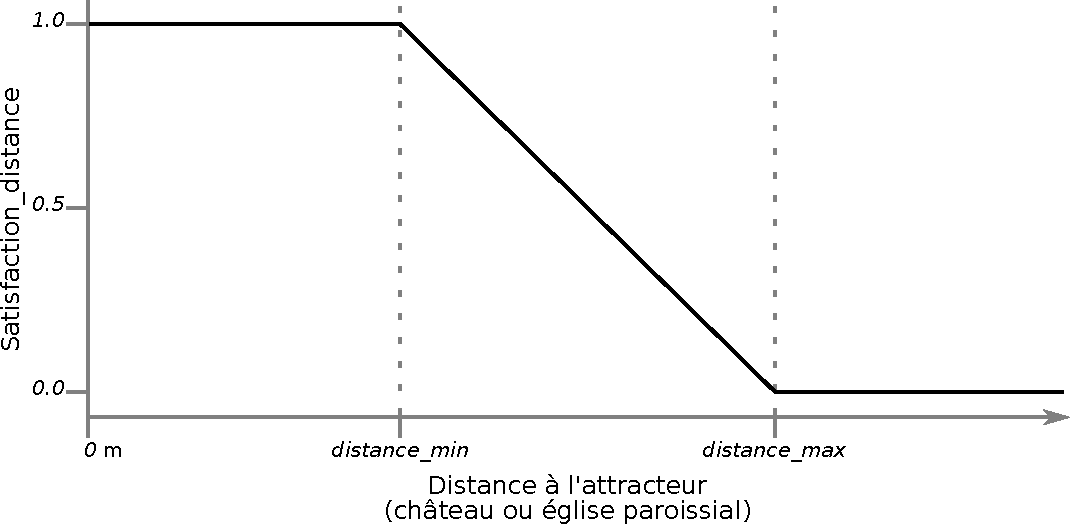
\includegraphics[width=.8\linewidth]{img/satisfaction_distance.pdf}
	\caption{Évolution de la satisfaction en fonction de la distance à l'attracteur le plus proche.}
	\label{fig:satisfaction-distance}
\end{figure}

\paragraph{Satisfaction religieuse}
		
Le calcul de la satisfaction religieuse s'inscrit rigoureusement dans cette logique.
On peut le formuler ainsi :
		\begin{equation*}
		s_{religieuse} = min  \left \lbrack max \left \lbrack \frac{(distance_{max} - distance\_eglise)}{(distance_{max} -distance_{min})}; 0 \right \rbrack ; 1 \right \rbrack
		\end{equation*}
avec les seuils de distance ($distance\_max$ et $distance\_min$) qui évoluent au cours du temps de telle manière :
\begin{itemize}
	\item avant 960 : $distance_{min}$ = 5 km et $distance_{max}$ =  25 km
	\item de 960 à 1060 : $distance_{min}$ = 3 km et $distance_{max}$ =  10 km
	\item après 1060 : $distance_{min}$ = 1,5 km et $distance_{max}$ =  5 km
\end{itemize}
	
\paragraph{Satisfaction protection}	

La satisfaction protection mobilise une logique proche, c'est-à-dire qu'elle est fonction de la distance au château le plus proche.
Cette distance est ici pondérée par un paramètre ($besoin\_protection$) qui permet de prendre en compte la réaction face à un climat de violence, lequel tend à augmenter pendant la période.

\begin{equation*}
s_{protection} = (s_{distance\_chateau})^{(besoin\_protection)}
\end{equation*}
avec
\begin{equation*}
\begin{gathered}
s_{distance\_chateau} = min  \left \lbrack
max \left \lbrack \frac{(dist_{max} - distance\_chateau)}{(dist_{max} -distance_{min})}; 0.01 \right \rbrack ; 1 \right \rbrack
\end{gathered}
\end{equation*}
($dist_{min}$ = 1,5 km et $dist_{max}$ = 5 km )
et le besoin de protection évolutif :
\begin{itemize}
	\item avant 960 : $besoin\_protection = 0 $
	\item de 960 à 1020 : $besoin\_protection = 0.2 ; 0.4 ; 0.6 ; 0.8$
	\item après 1020 : $besoin\_protection = 1$
\end{itemize}

\paragraph{Satisfaction matérielle}

La satisfaction matérielle ne prend aucune distance en compte : elle s'appuie sur le montant des taxes dont le foyer paysan doit s'acquitter ($redevance\_acquittees$).
Ce montant est pondéré par un paramètre technique représentant un niveau \og acceptable\fg{} de taxation ($coef\_redevances$, qui vaut $15$ ici).
L'appartenance du foyer paysan à une communauté fini de contre-balancer le montant des redevances acquittées, sous la forme d'un contre-poids dont l'importance augmente au fur et à mesure de la période modélisée ($puissance\_communaute$ vaut $0.2$ jusqu'en 1060, puis augmente de $0.2$ à chaque pas de temps pour atteindre $1$ en 1040 et rester à ce niveau).

\begin{equation*}
\begin{gathered}
s_{materielle} = (s_{redevance})^{(1-puissance\_communaute)}
\end{gathered}
\end{equation*}
avec 
\begin{equation*}
\begin{gathered}
s_{redevance} = max \left[ \left( 1- \frac{redevances\_acquittees}{coef\_redevances} \right) ; 0 \right]
\end{gathered}
\end{equation*}

\paragraph{Satisfaction générale}

La satisfaction générale est mesurée en prenant le minimum de ces satisfaction individuelles, c'est-à-dire qu'on considère qu'elles ne s'équilibrent pas.
Comme pour la satisfaction matérielle qui la compose, l'appartenance du foyer paysan à une communauté paysanne tend aussi à augmenter la satisfaction générale.
Les communautés interviennent donc à deux reprises dans le calcul de la satisfaction, afin d'illustrer le poids que prennent ces structures sociales et institutionnelles au cours de la période modélisée.

Le calcul de la satisfaction s'exprime ainsi :
\begin{equation*}
\begin{gathered}
\begin{split}
satisfaction =~& 0.75 \times \left[ min \left( s_{materielle} ; s_ {religieuse}; s_{protection} \right) \right] + \\
& 0.25 \times [appartenance\_communaute]
\end{split}
\end{gathered}
\end{equation*}
avec $ \{satisfaction ; s_{materielle} ; s_ {religieuse} ; s_{protection}\} \in [0,1]$ et $[appartenance\_communaute] \in \{0;1\} $


	\subsubsection{Migration des foyers paysans \label{sssec:migration}}

La migration des foyers paysans est sans doute le mécanisme le plus complexe et ayant subi les plus fortes évolutions depuis la conception de SimFeodal.
La règle d'ensemble est pourtant extrêmement simple : un foyer paysan a une probabilité de migrer qui est inversement proportionnelle à sa satisfaction. 
Autrement dit, $P \left( migration \right) = \left( 1 - satisfaction \right)$.
Cette règle simple a été progressivement complexifiée afin d'augmenter la rationalité et l'ancrage empirique des choix de localisation.
Une première complexification a abouti à la distinction de migrations \og locales\fg{} et de migrations \og lointaines\fg{} (voir \cref{fig:migrations-locales-lointaines}).

\begin{figure}[H]
\centering
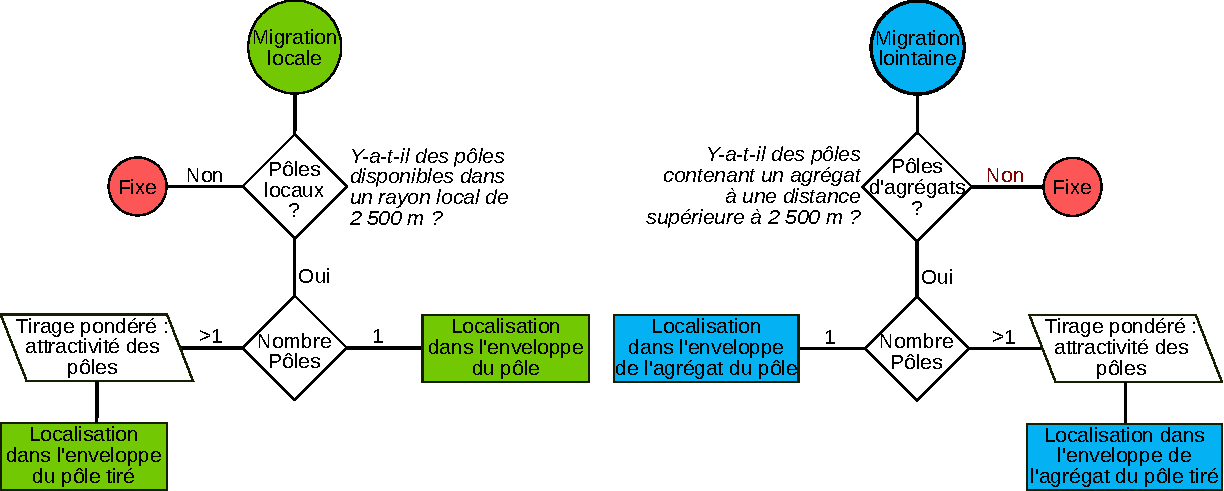
\includegraphics[width=1\linewidth]{img/migration_locale-lointaine.pdf}
\caption{Migrations locales et lointaines.}
\label{fig:migrations-locales-lointaines}
\end{figure}
Pour aboutir à cette différence entre migration locale et migration lointaine, la règle est encore une fois complexe : les foyers paysans privilégient les migrations locales, et quand celles-ci ne sont pas possibles, ils ont une probabilité plus faible d'effectuer une migration lointaine.
Notons que pour nous approcher des connaissances empiriques, nous avons établi un comportement légèrement différent entre les foyers paysans déjà agrégés et ceux qui seraient dispersés lors de l'exécution du mécanisme de migration (\cref{fig:choix-migration}).
\begin{figure}[H]
	\centering
	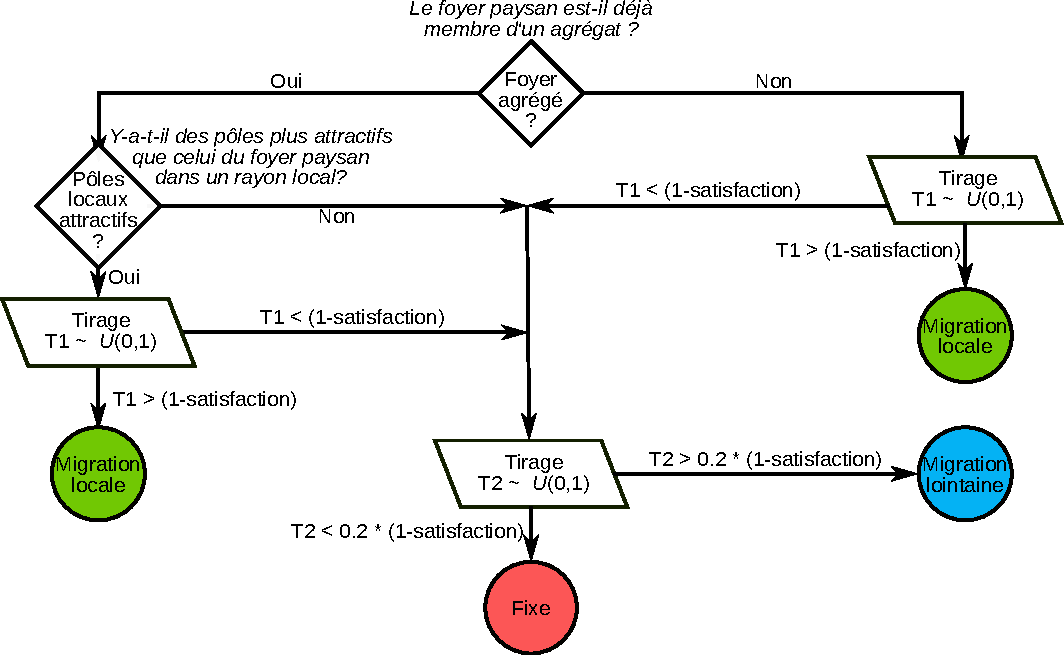
\includegraphics[width=0.9\linewidth]{img/choix_migration.pdf}
	\caption{Décision de migration.}
	\label{fig:choix-migration}
\end{figure}

Une dernière distinction a été opérée entre les foyers paysans classiques, libres de leurs migrations, et les foyers paysans \og dépendants\fg{}.
Ces derniers représentent les foyers qui n'avaient pas le droit de quitter le domaine de leur seigneur (les serfs entre autres).
Ceux-là ne peuvent effectuer que des migrations locales, et on considère qu'ils seront amenés à migrer plus facilement, ce qui change encore une fois leur mécanisme de migration (\cref{fig:choix-migration-dependants}).
\begin{figure}[H]
	\centering
	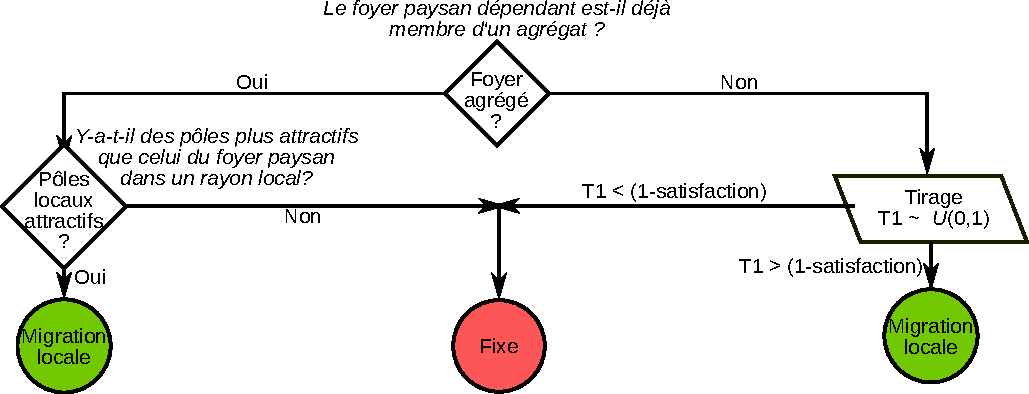
\includegraphics[width=0.9\linewidth]{img/choix_migration_dependants.pdf}
	\caption{Décision de migration des foyers paysans dépendants.}
	\label{fig:choix-migration-dependants}
\end{figure}
 

	
\subsection{Seigneurs}
	\subsubsection{Prélèvement des droits \label{sssec:collecte-droits}}
\setcounter{footnote}{\value{savefootnote}}
Les seigneurs, petits et grands, collectent les droits dont doivent s'acquitter les foyers paysans (droits de haute justice et autres droits) majoritairement (exception faite des droits fonciers pour les grands seigneurs, voir \cref{fig:prelevement-fonciers}) par l'intermédiaire des zones de prélèvement.
Ces zones sont caractérisées par un propriétaire (le seigneur qui les possèdent), éventuellement un gardien (le seigneur à qui la zone a été \og donnée\fg{}, voir \cref{meca-dons}), une localisation\footnote{Pour les petits seigneurs, il s'agit de leur propre localisation}, un rayon\footnote{
Ce rayon est tiré aléatoirement suivant une distribution uniforme, \\$rayon\_zp \sim \mathcal{U}\left[ rayon\_min\_zp\_ps , rayon\_max\_zp\_ps \right]$, avec $rayon\_min\_zp\_ps$ et $rayon\_max\_zp\_ps$ des paramètres qui valent respectivement 1 000 et 5 000 m.
} et un taux de prélèvement\footnote{
idem : $taux\_prelevement\_zp \sim \mathcal{U}\left[ min\_taux\_prelevement\_zp\_ps , max\_taux\_prelevement\_zp\_ps \right]$ avec $min\_taux\_prelevement\_zp\_ps$ et $max\_taux\_prelevement\_zp\_ps$ valant 5\% et 25\%.
}.
À noter que les zones de prélèvement liées à des châteaux suivent une règle légèrement différente, que nous n'aborderons pas ici\footnote{Se référer au code-source du modèle, dans la fonction \textsf{construction\_chateaux}}.

Les prélèvements, selon les types de droits, rapportent de la \og puissance\fg{} aux seigneurs, dont le \cref{tab:puissance-droits} donne une référence.

\begin{table}[H]
	\centering
	\caption{Gain de puissance par foyer paysan prélevé.}
	\label{tab:puissance-droits}
	{\renewcommand{\arraystretch}{1.1}%
		\begin{tabular}{|l|l|l|}\hline
			\textbf{Type de droit} & \textbf{Fonction du seigneur} & \textbf{\makecell{Puissance acquise\\par foyer paysan}} \\ \hline
			\multirow{2}{*}{Haute Justice} & Propriétaire ou Gardien & 2 \\
			& Souverain (zone donnée) & 2.5 \\ \hline
			\multirow{2}{*}{Droits fonciers} & Propriétaire ou Gardien & 1 \\
			& Souverain (zone donnée) & 1.25 \\ \hline
			\multirow{2}{*}{Autres droits} & Propriétaire ou Gardien & 0.25 \\
			& Souverain (zone donnée) & 0.35 \\ \hline	
	\end{tabular}}
\end{table}


\paragraph{Foncier}

Quelques petits seigneurs (ceux créés dès l'initialisation ainsi que $\approx 10\%$ de ceux créés pendant le déroulement de la simulation) possèdent des droits fonciers.
À ce titre, ils peuvent collecter ces droits au sein d'une zone de prélèvement qu'ils créent lors de leur apparition.
Le mécanisme de collecte des droits fonciers est illustré dans la \cref{fig:prelevement-fonciers}.
\begin{figure}[H]
	\centering
	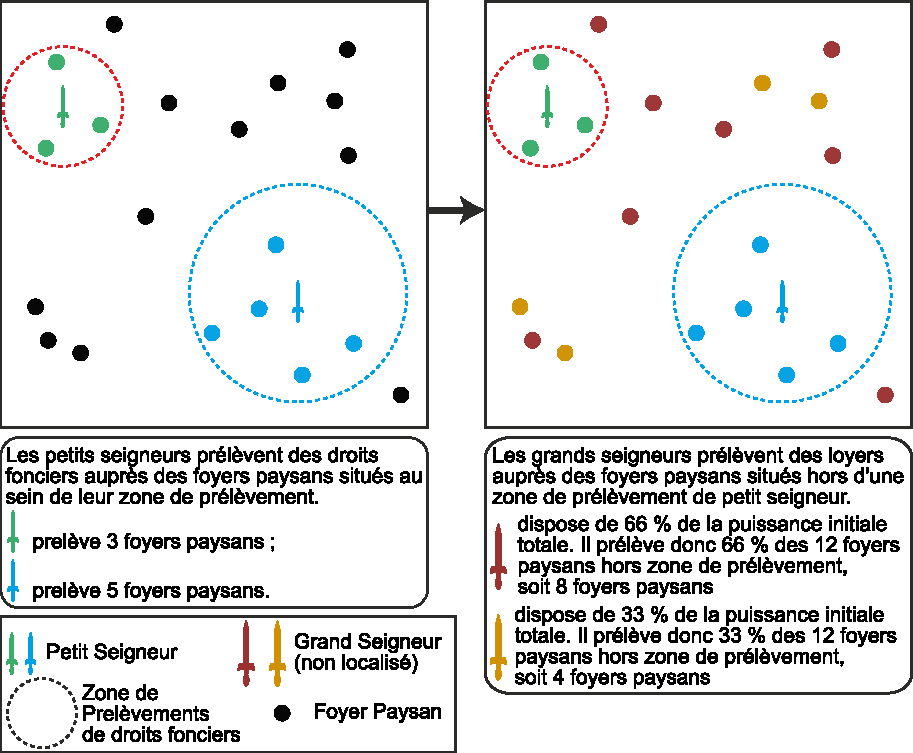
\includegraphics[width=0.8\linewidth]{img/prelevements_foncier.pdf}
	\caption{Prélèvement des droits fonciers par les petits et grands seigneurs.}
	\label{fig:prelevement-fonciers}
\end{figure}

\paragraph{Haute justice et autres droits}

Les autres droits suivent un mécanisme plus générique : les seigneurs propriétaires collectent des droits auprès d'une partie des foyers paysans inclus dans la surface de la zone de prélèvement.
Cette partie correspond aux \og taux de prélèvement\fg{} décrit plus haut. La \cref{fig:prelevement-droits} récapitule les différentes modalités de collecte de droits via les zones de prélèvement.

\begin{figure}[H]
	\centering
	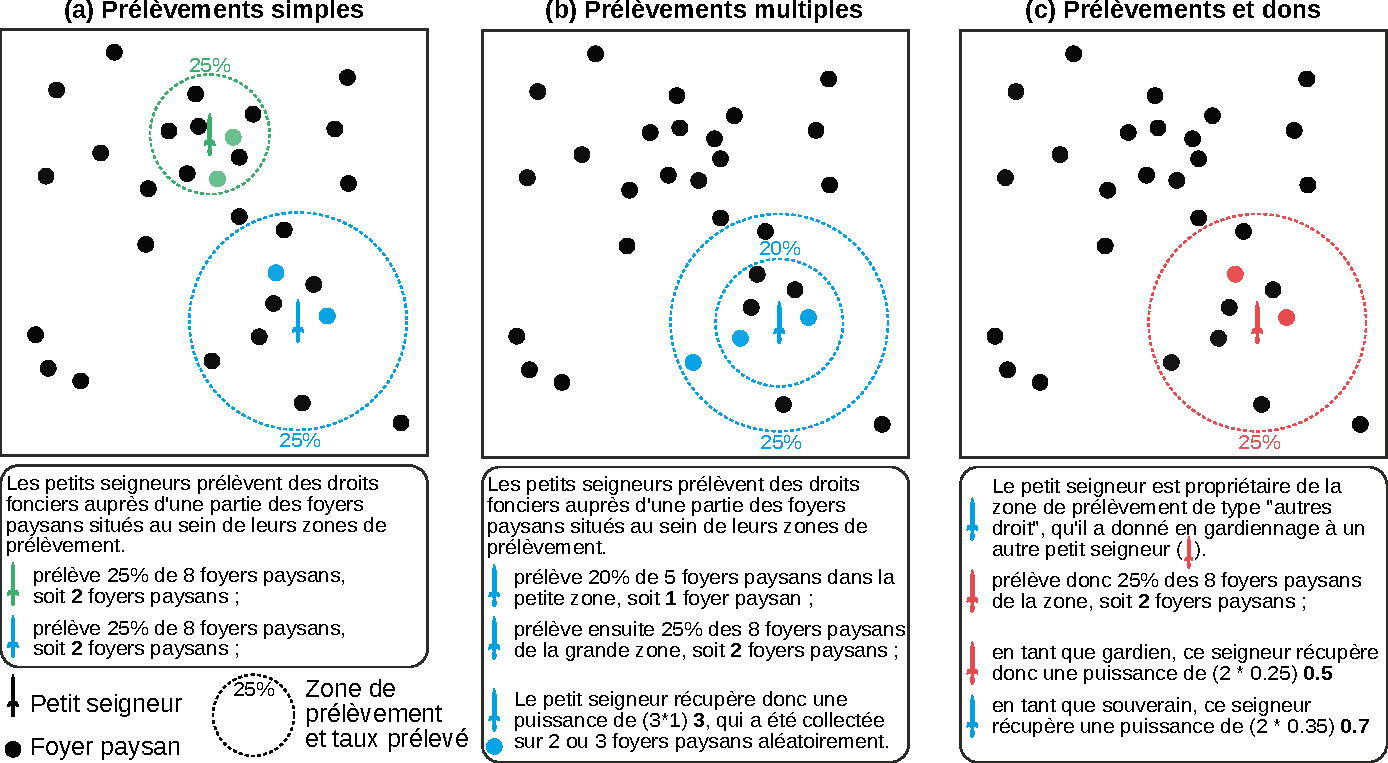
\includegraphics[width=\linewidth]{img/prelevements_droits.pdf}
	\caption{Mécanisme général de prélèvement des droits par les seigneurs.}
	\label{fig:prelevement-droits}
\end{figure}

Les droits de haute justice sont prélevés exactement comme les autres droits, à la seule différence qu'ils correspondent nécessairement à des taux de prélèvement de 100\%.

\subsubsection{Construction de châteaux \label{sssec:constru-chateaux}}


À partir de 940, les seigneurs ont la possibilité de créer des châteaux.
Le mécanisme de construction des châteaux est commun aux grands et aux petits seigneurs, mais certains paramètres varient selon le type du seigneur considéré :
\begin{itemize}
	\item Un grand seigneur peut construire jusqu'à $2$ châteaux par tour (paramètre $nb\_max\_chateaux\_par\_tour\_gs$), alors qu'un petit seigneur ne peut en construire au maximum que $1$ par pas de temps ($nb\_max\_chateaux\_par\_tour\_ps$).
	\item Pour un seigneur $i$, la probabilité de construire un château est formalisée ainsi :\\
	$$ P \left( construction \right) =  \frac{puissance\_seigneur_{i}}{\sum{puissance\_seigneur_{0..n}}} \times ponderation\_proba\_chateau $$ avec $ponderation\_proba\_chateau$ valant $1.25$ pour les grands seigneurs et $7$ pour les petits (paramètres techniques).
	\item Les grands seigneurs peuvent construire des châteaux n'importe-où dans l'espace du modèle (en respectant toutefois les règles exposées plus bas), alors que les petits seigneurs ne peuvent le faire que dans un rayon de 5 000 m de leur localisation : s'il n'y a pas d'espace disponible dans ce rayon, le petit seigneur ne crée pas de château.
\end{itemize}

Les règles de localisation de château sont identiques, et illustrés dans la \cref{fig:construction-chateaux}.

\begin{figure}[H]
	\centering
	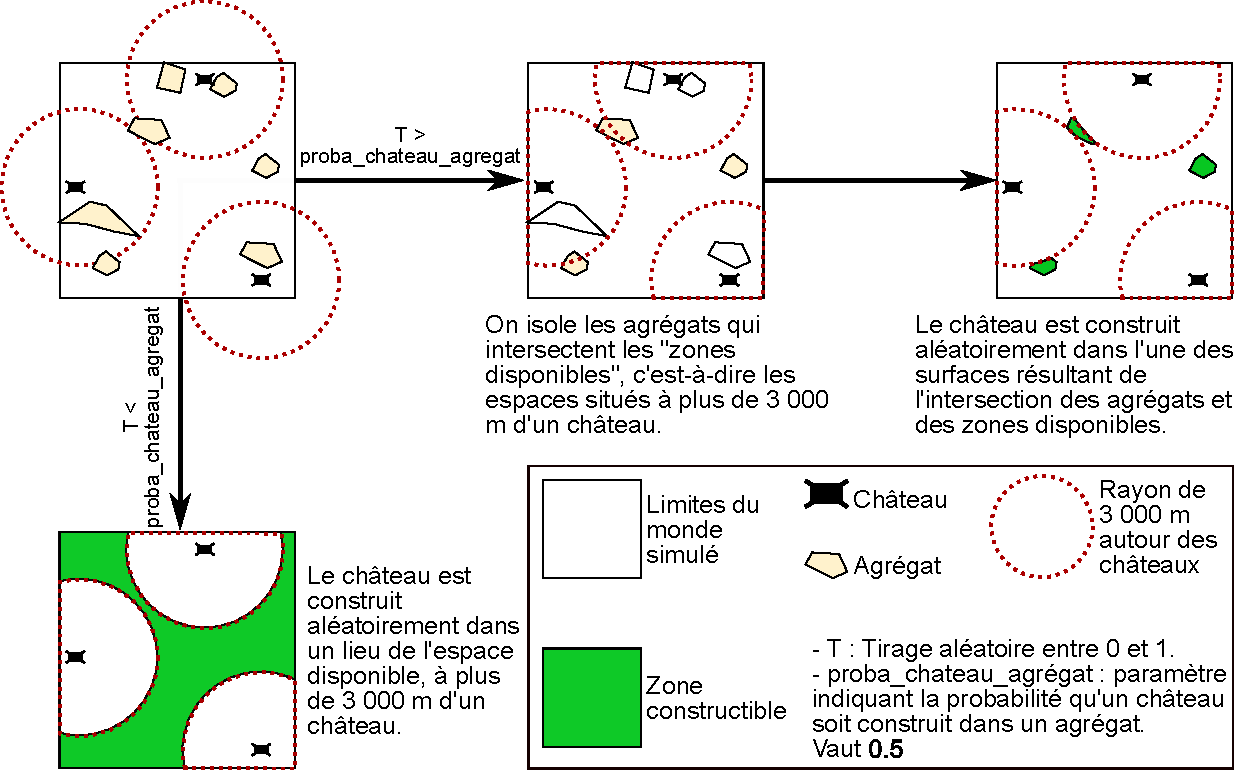
\includegraphics[width=\linewidth]{img/construction_chateaux.pdf}
	\caption{Mécanisme de localisation des châteaux construits.}
	\label{fig:construction-chateaux}
\end{figure}

\paragraph{Rayon des zones de prélèvement associées}

La construction d'un château implique systématiquement la création de zones de prélèvements qui lui sont associées, c'est-à-dire qu'elles appartiennent au seigneur qui crée le château.
Si le château est donné en gardiennage, l'ensemble des zones de prélèvement qui lui sont associées seront aussi données en gardiennage au petit seigneur choisi.

Les zones de prélèvement créées concernent des droits fonciers et des autres droits.
Si le seigneur châtelain obtient les droits de haute justice, une zone de prélèvement de droits de haute justice sera automatiquement créée autour de chacun de ses châteaux.
Contrairement aux zones de prélèvement habituelles, celles qui sont associées à un château ont un taux de prélèvement de $100\%$.
Leur rayon est variable et dépend de la puissance relative du seigneur qui construit le château.
Ce rayon varie entre un seuil minimal de 2 000 m ($rayon\_min\_zp\_chateau$) et un seuil maximal de 15 000 m ($rayon\_max\_zp\_chateau$).
Entre ces deux seuils, la valeur du rayon dépend d'une fonction linéaire correspondant au ratio entre la puissance du seigneur constructeur et les puissances maximales et minimales de l'ensemble des seigneurs, tel que formalisé dans l'équation \ref{eq:rayon-zp-chateau}. 

\begin{equation}\label{eq:rayon-zp-chateau}
\begin{aligned}
& rayon\_zp\_chateau = \\
& min  \left[ max \left[ puissance\_relative; rayon\_min\_zp\_chateau \right]  ; rayon\_max\_zp\_chateau \right]
\\
& \text{avec}
\\
& puissance\_relative_i = \frac{max(puissance_{0..n}) - puissance_i}{max(puissance_{0..n}) \times min(puissance_{0..n})}
\end{aligned}
\end{equation}

\section*{Conclusion}
\addcontentsline{toc}{section}{Conclusion}

\hl{À rédiger}

\begin{itemize}
	\item Reprise processus de modélisation exploratoire.
	\item -> Nombreux changements, étalé sur un temps semi-long (+ 5 ans (21/04/2014) depuis le premier commit, qui donnait déjà une première version fonctionnelle du modèle), travail commencé avec moi en réunion en mars 2013, pour le séminaire TMD de Sommières de Juin 2013, soit avant le début de cette thèse. 
	\item -> Hétérogénéité forte dans le niveau de détail des mécanismes
	\item Description ni complète, ni trop schématisée : une tentative de juste milieu, qui respecte le niveau de détail de chacun des mécanismes.
\end{itemize}





\printbibliography[title={Références}]
